\documentclass[10pt,a4paper,twocolumn]{article}
\usepackage{bachelorproject}

\title{\vspace{-0.5in}{\bfseries\scshape 
    Connectionist Reinforcement Learning to Contain Forest Fires
    } \\ 
    \vspace{1ex} 
    \normalsize{Bachelor's Project Thesis}\vspace{-2ex}
}

\author{
    \normalsize{Travis Hammond, s2880024, dashdeckers@gmail.com,} \\ 
    \normalsize{Supervisor: Prof Marco Weiring}
}

% Table of Contents:


% Introduction
%% Forest Fires
%% Reinforcement Learning

% Methods
%% Environment
%%% Fire Spread
%%% Reward Function
%%% State Representation
%% Agent
%%% Problems
%%% Experience Replay
%%% Target Network
%%% QL vs SARSA
%%% Duelling
%%% Demo Data
%%% Experiment Setup

% Results

% Conclusion

\date{\vspace{-5ex}}


\begin{document}

\twocolumn[
  \maketitle
  \begin{@twocolumnfalse}
    \begin{abstract}
{With global temperatures on the rise, forest fires are becoming more frequent and forest fires, in turn, contribute to global warming by releasing large amounts of CO2 into the atmosphere and eliminating the trees that would be able to process the CO2. Finding a way to effectively control and contain these fires is therefore becoming more and more of a priority.
In this paper, we propose a connectionist reinforcement learning system that can learn to contain the spread of a simulated fire. It can do this by cutting fire lines around the fire, removing the fuel needed for it to spread further.
We show the performance of a connectionist Q-Learning algorithm with a target network and experience replay, and compare it to three more implementations. One that uses the on-policy algorithm SARSA, one with the addition of a dueling network architecture and one with both modifications.
To accelerate learning, we use a vision grid approach in which the system receives as input three versions of the full map size each showing only a single feature such as agent location and fire locations. We also provide the algorithm with different amounts of demonstration data.
The results show the ability of each proposed system to successfully contain the fire within a reasonable number of training episodes. Both modifications have their advantages and disadvantages with regard to reliance on demonstration data and learning stability.

\vspace{6ex}}
\end{abstract}

  \end{@twocolumnfalse}
]

\thispagestyle{firststyle}

%!TEX root = report.tex

\section{Introduction}\label{sec:introduction}

\subsection{Forest Fires}
The ever increasing temperature around the globe due to global warming brings many consequences. One of which is the increased risk of forest fires. Warmer climates are plagued by forest fires not only more frequent, but also more intense.  In most cases, beginning wildfires are extinguished before they get out of hand. Sadly, some wildfires escalate into nearly uncontrollable infernos.

Fighting these forest fires is a challenging task. To extinguish a fire one or more of the three required elements has to be eliminated: fuel, heat or oxygen. The ordinary tactic is to remove the heat and oxygen by spraying water or foam from hoses, but large forest fires require more effort to be contained. Possible options include aircrafts dropping water bombs, burning down specific areas in a controlled fashion, or using a bulldozer to cut fire lines. The use of these techniques need to be carefully planned by the fire-fighters when constructing a plan. To create the perfect plan is a near impossible job and it is not uncommon for plans to fail and cause the loss of more forest.

Not only can forest fires result in the tragic loss of lives and houses, the ecological effect has to be taken into account as well. Trees and plants are a key factor in the carbon cycle \citep{kasischke1995fire}. Using photosynthesis massive amounts of CO$_{2}$ are filtered from the atmosphere and stored. When fires destroy large forests, all this stored CO$_{2}$ is released back into the atmosphere, which is inconsistent with the carbon cycle. Since this CO$_{2}$ is considered a greenhouse gas \citep{houghton1991climate} which boosts the already increasing global warming, this will increases the likelihood and risk of forest fires. The just described relationship has the potential to result in a dangerous cycle with grave consequences for the eco system as well as for the habitability of the planet for humans.

In light of the seriousness of the problem there is still not much research being done in the field of artificial intelligence to optimize the coordination of fire fighting efforts. Previous research mostly focussed on the detection and prediction of forest fires, but exceptions include investigations into how to construct a simulator for forest fires and how reinforcement learning algorithms could optimise policies by interacting with such a simulation \citep{wiering1998learning}, research exploring how enforced sub-populations (ESP) could be used to evolve neural network controllers capable of solving the forest fire problem \citep{wiering2005evolving}, and a model of multi-agent coordination in fire fighting scenarios \citep{moura2007fighting}.

In this paper we explore how connectionist reinforcement learning (RL) can be used to allow an agent to learn how to contain forest fires in a simulated environment by using a bulldozer to cut fire lines. We make use of existing algorithms: $Q$-Learning \citep{watkins1989learning}, SARSA \citep{rummery1994line} and Dueling $Q$-Networks \citep{wang2015dueling}. We show that using a simple baseline algorithm to generate demonstration data to be used in experience replay can greatly increase the algorithm's performance. We show that these algorithms are able to complete this task successfully in small simulations. We also introduce a new RL algorithm, Dueling SARSA, which combines the latter two and outperforms all, especially in simulations of a larger size where others fail.

Our research question is: Does connectionist $Q$-Learning or SARSA, both with or without the dueling network architecture, perform better at containing the spread of a simulated forest fire by cutting fire lines in a simulated environment?

\subsection{Reinforcement Learning}\label{sec:reinforcementlearning}
Reinforcement learning is a machine learning paradigm typically consisting of two elements. The first is the agent, which represents the reinforcement learning algorithm, and the second is the environment, which represents what the algorithm is trying to solve. This is typically a game or in this case, a simulated forest fire that should be contained.

At each discrete time step $t \in \{1,2,3...,T\}$, the environment provides the agent with an observation $s_t \in \mathcal{S}$. Then, the agent interacts with the environment by choosing an action $a_t$ from a limited set of possible actions $\mathcal{A}=\{1,...,K\}$, and observes the result of that action in state $s_{t+1}$ and the obtained reward $r_t$. This interaction can be modelled by a Markov Decision Process, or MDP, as long as the Markov property holds: The probability of state $s_{t+1}$ only relies on the previous state $s_t$ and the performed action $a_t$. This property indeed holds, as the simulation only requires the current state and agent action to produce the next state.

The goal of the agent is to select actions in a way that maximizes the cumulative future reward from the current time step $t$, which is defined as:
\begin{equation}\label{eq:cumulative_reward}
	R_t = \sum_{t'=t}^{T} \gamma^{t'-t} r_{t'},
\end{equation}
where $T$ is the time-step at which the game terminates and $\gamma \in [0,1]$ is a discount factor that determines the trade-off between the importance of immediate and delayed rewards. 

A policy $\pi$ is a mapping of states to actions (or distribution over actions). To determine the optimal policy $\pi^*$, that leads to the highest reward as defined in Equation \eqref{eq:cumulative_reward}, we define the optimal action-value function (also known as $Q^*$) to be:
\begin{equation}\label{qfunction}
	Q^*(s, a) = \max_\pi \sum_{t=1}^T [r_t \vert s_t=s, a_t=a, \pi]
\end{equation}

We can estimate this $Q$-function using temporal difference and dynamic programming methods through iterative updates to the Bellman equation
\begin{equation}
	\begin{array}{c}
		Q_{i+1}(s, a) = \sum_{s'} P(s' \vert s, a) [R(s,a,s') + \\
		\gamma \max_{a'} Q_i(s', a')],
	\end{array}
\end{equation}
where $P(s'\vert s,a)$ is the probability of observing state $s'$ after executing action $a$ in state $s$, and $R(s,a,s')$ is the reward obtained after executing action $a$ in state $s$ and ending up in state $s'$.
Such a value iteration algorithm will eventually converge to the optimal $Q$-function $Q^*$ as $i \rightarrow \infty$. From this function, the optimal policy can easily be derived by simple taking the highest-valued action in each state. In connectionist reinforcement learning, it is common to approximate this function using a neural network
\begin{equation}
	Q(s, a; \theta) \approx Q(s, a),
\end{equation}
where $\theta$ are the parameters, or weights, of the $Q$-Network.
\section{Methods}\label{sec:methods}

\subsection{Environment}\label{sec:environment}
a basic rundown of the simulation, how it works

\subsubsection{Fire Spread Dynamics}\label{sec:fire_spread}
specifically the fire spread dynamics

\subsubsection{The Reward function}\label{sec:reward_function}
The reward function is a function that maps each state to a value that represents how "good" or desirable that state is. As such, this function is a vital part of the learning process because any reinforcement learning algorithm will rely on two things because they constitute the input to the agent (See basic RL schema). The quality of the state representation, or in other words how much of- and how well the agent sees the environment, and the quality of the reward function, or how well the agents notion of success corresponds with our notion of success and how easy it is to find optima in the reward landscape.

Apart from determining the optimal policy to be learned by the agent, the reward function also determines the speed at which the agent will be able to learn that policy. To take the gradient descent analogy of a problem landscape, if the reward function produces a smooth gradient to the optimal solution, the agent will be able to find a path to that solution more easily than if the reward resembles flat landscape with sparse spikes in which the value jumps from almost always 0 or negative to a positive reward. In other words, the agent should be provided gradual feedback instead of sparse rewards in order to facilitate fast and efficient learning.

Crafting a good reward function for this problem turned out to be quite difficult because it was hard to define a measure of success that is both valid in its formulation and which provides gradual feedback, or a smooth gradient, towards the containment of the fire. We defined the reward function as
\[
R = \left\{\begin{array}{lr}
    1000, & \text{ Fire is contained }\\
    1000 * (p), & \text{ Fire burns out }\\
    -1000, & \text{ Agent dies }\\
    -1 & \text{ Otherwise }

    \end{array}\right\}
\]
where~$p$ is the percent of the map undamaged by either fire or digging. We decided to choose a reward function that defines the goal well, and then compensate for the lack of a smooth gradient with demonstration data to lead it towards the sparse rewards. Note that the 2nd and 3rd states are the only terminal states.

Containment of the fire is determined by (Link to algorithm). The algorithm returns true as soon as it can find a path, not allowing diagonal movements, between any burning cell and any cell on the border of the map. It uses the A* path-finding algorithm to check for a path between any two points.

% Pseudocode for the containment algorithm


\subsubsection{The State Representation}\label{sec:state_rep}
The state of the environment, or the observation of the environment as it is visible to the agent, consists of 3 matrices of size N*M with a boolean domain resulting in, after flattening, an array of (3 * N*M) boolean inputs where (N, M) are the dimensions of the map. Assuming the shape of the map is always square, a map size of (N=10) elements is represented three times: One layer contains only the agent position, translating to a matrix of zeros except for a single one representing the position of the agent. The second layer consists of the position of the fire. Cells that are on fire are represented by a 1, the rest are set to 0. The third layer represents the fire lines cut by the agent in a similar boolean fashion, resulting in a total of 300 inputs to the agent. This is schematically shown in \ref{fig:visiongrid}.

\begin{figure}[h]
    \centering
    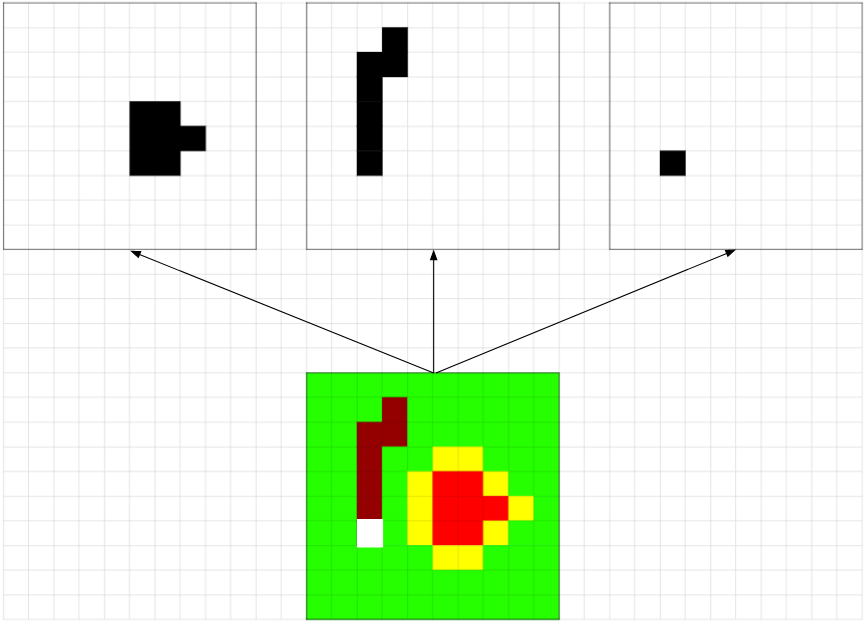
\includegraphics[width=1\linewidth]{img/Vision_Grid.png}
    \caption{A vision grid representation of an example state}
    \label{fig:visiongrid}
\end{figure}

This vision grid approach can speed up the learning process as well as increase the performance (citation Opponent Modelling in the Game of Tron using Reinforcement Learning). Indeed it had a noticeable effect on the performance and learning speed of our implementation compared to a single matrix representing the gray-scaled map as input, likely because the agent can more easily differentiate between different attributes and because only the relevant information is presented. Further, the agent can now see whether the cell it is occupying is already dug or not.


\subsection{The Agent}\label{sec:agent}


\subsubsection{Known Problems with Connectionist RL}\label{sec:problems}
The combination of function approximation (the neural network), bootstrapping (TD methods that update Q-values using estimated return values) and off-policy training (the Q-Learning algorithm) make up the deadly triad \citep{sutton_barto_2018}, which is known to cause instabilities and even divergence in the learning process. There are two well known strategies to reduce this effect and stabilise learning, using experience replay and a target network \citep{mnih2015human}.

\subsubsection{Experience Replay}\label{sec:exp_replay}

\begin{figure}[h]
    \centering
    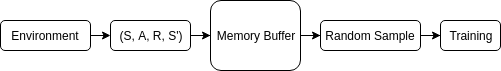
\includegraphics[width=1\linewidth]{img/Experience_Replay.png}
    \caption{Schematic structure of experience replay}
    \label{fig:expreplay}
\end{figure}

Instead of training the network on incoming experiences directly, the experiences can be stored in a memory buffer and the network can be trained on a mini-batch of memories randomly sampled from this buffer (see \ref{fig:expreplay}). This helps because neural networks assume that each training sample is identically and independently distributed with regard to the population the algorithm is set up to approximate (Citation needed), and training directly on incoming experiences break this assumption in two regards.

For one, consecutive incoming experiences are obviously highly correlated because the environment does not radically change after any action (unless it leads to a terminal state). This means that any experience differs from the previous experience only to the extent to which the environment can change in one update step from a single action from the agent. (Citation needed)

The distribution of incoming experiences is also dependent on the agents current policy. If the current policy determines that the agent should head east, then the next experiences recorded by the agent will involve the agent headed east. Apart from the obvious correlation, this can also lead to feedback loops (Explain the loops and cite dqn + paper below)

% https://arxiv.org/pdf/1511.05952.pdf
%(Check out the link for good reasons why experience replay is useful. already in .bib file)

\subsubsection{Target Network}\label{sec:target_network}
Another source of instability is that we use the predictions of the network to generate the target values which, combined with the rest of the update rule which will be explained in the next section, directly update the weights of that same network. This can lead to unwanted feedback loops. We can add a delay to the loop to reduce these effects by using a periodically updated, frozen copy of the network to generate the target values instead (as shown in \ref{fig:targetnet}). Every C iterations, the target network is replaced by a copy of the main network. This modification is called Double Q-Learning \citep{NIPS2010_3964}, and was also used by \citep{mnih2015human} to make the algorithm more stable and prevent divergence.

\begin{figure}[h]
    \centering
    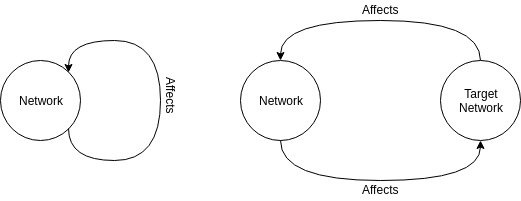
\includegraphics[width=1\linewidth]{img/Target_Network.png}
    \caption{Highlighting the schematic difference of using a target network}
    \label{fig:targetnet}
\end{figure}


\subsubsection{Q-Learning vs SARSA}\label{sec:ql_sarsa}

\subsubsection{Duelling Networks}\label{sec:duelling}

\subsubsection{Demonstration Data}\label{sec:demo_data}
Because the reward function defined earlier provides sparse rewards, the agent needs additional guidance to fast track the learning process. To point it to the right direction, we can fill the memory buffer with human demonstration data before learning. However, this takes a lot of time to do by hand a sufficient number of times and can be automated. To this effect, the pseudocode in (figure so and so) was developed: It randomly picks from a set of two actions which depend on the position of the agent relative to the fire such that the agent will always move in a clockwise motion around the fire. As soon as the containment bonus is collected the environment resets, and this is continued until that bonus has been collected a specified number of times.
% pseudocoooode

\section{The Experimental Setup}\label{sec:experiment}
How were the results collected, which runs were done with which parameters etc

% Insert the algorithm
\begin{algorithm}
  \caption{Baseline algorithm to contain the fire}
  \label{baseline_algo}
  \begin{algorithmic}[1]
    \Procedure{RunBaseline}{}
    \State $totalreward = 0$
    \While {\textbf{not} $done$}
    \State {$action =$ random(possible actions)}
    \If {$action$ is dangerous}
    \State {$action =$ other possible action}
    \EndIf
    \State {$reward, done =$ execute(action)}
    \State $totalreward = totalreward + reward$
    \EndWhile
    \State \Return $totalreward$
    \EndProcedure
  \end{algorithmic}
\end{algorithm}

%!TEX root = report.tex

\section{Results}
It should be noted that all four algorithms are color-coded consistently throughout the plots. The lines represent averages of 10 training runs. The error bars are based on the standard error at that point in time. All tables are based on the final 2500 episodes of these 10-run averages.
\subsection{10-by-10 simulations}
% FIGURES 10-sized
\begin{figure}[H]
    \centering
    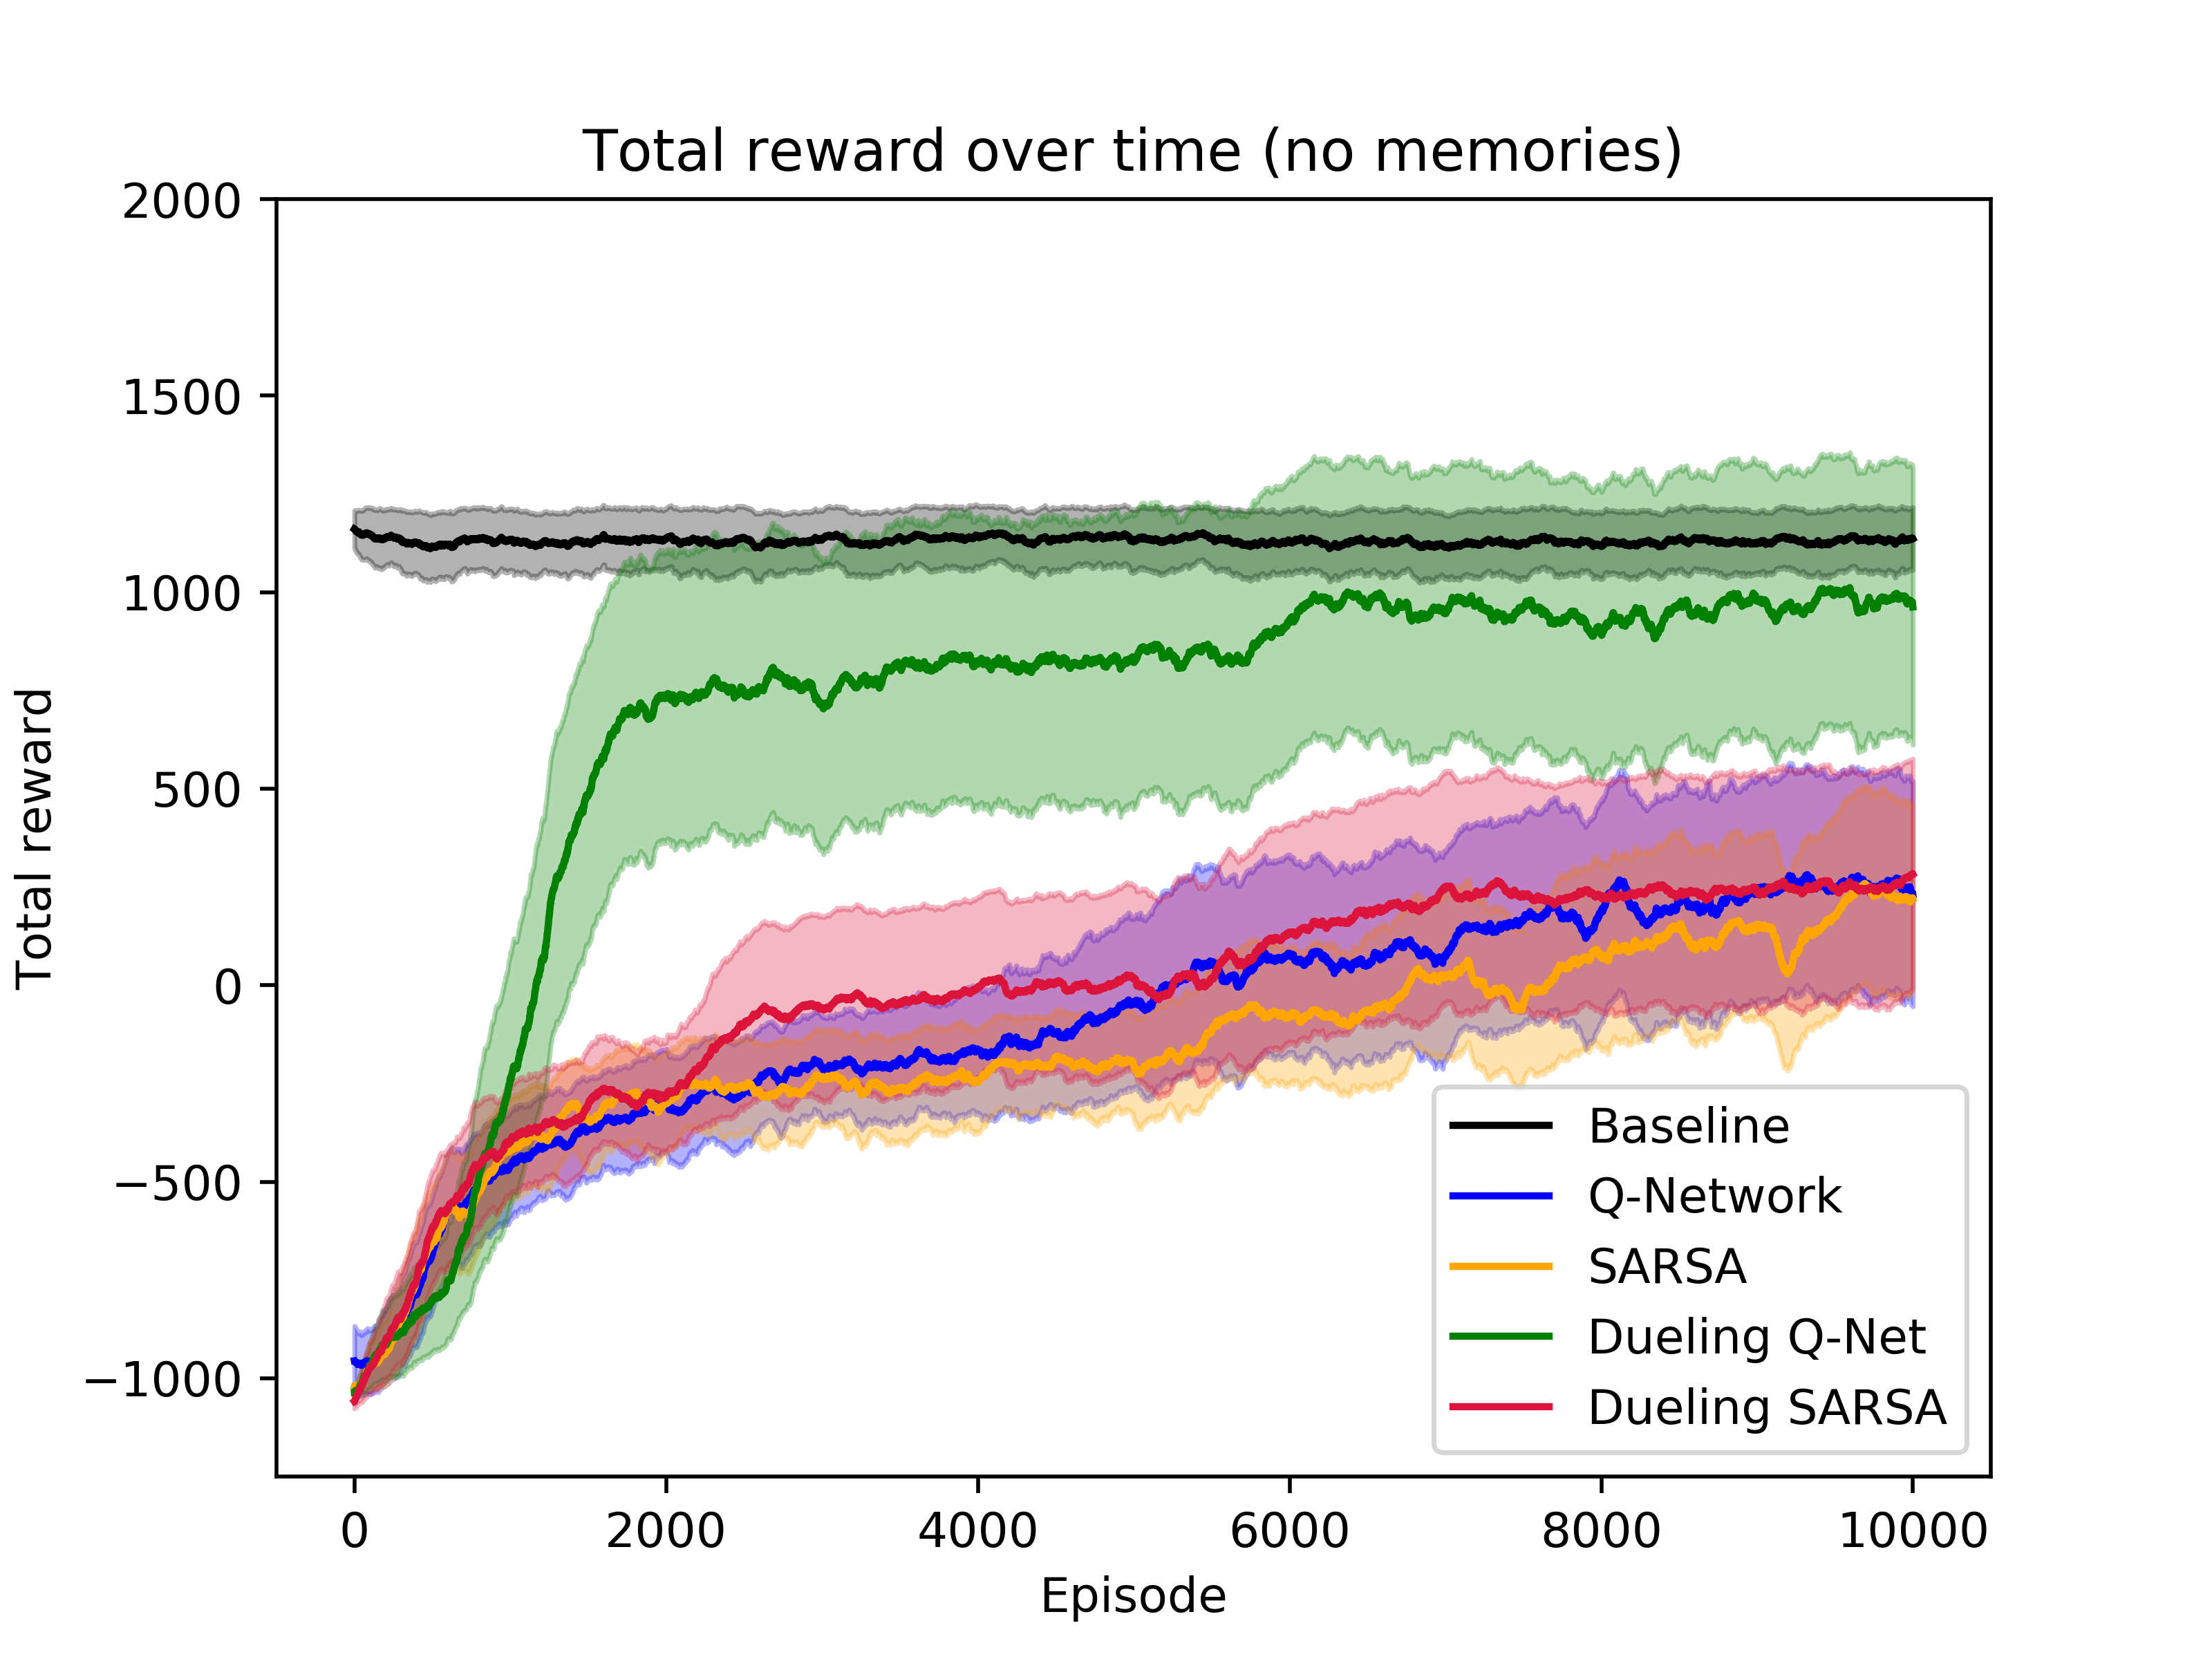
\includegraphics[width=\linewidth]{img/results/10-sized/total_rewards_0m-min.png}
    \caption{10-run averages given 0 episodes of demonstration data.}
    \label{fig:10sized-0mem}
\end{figure}
\begin{figure}[H]
    \centering
    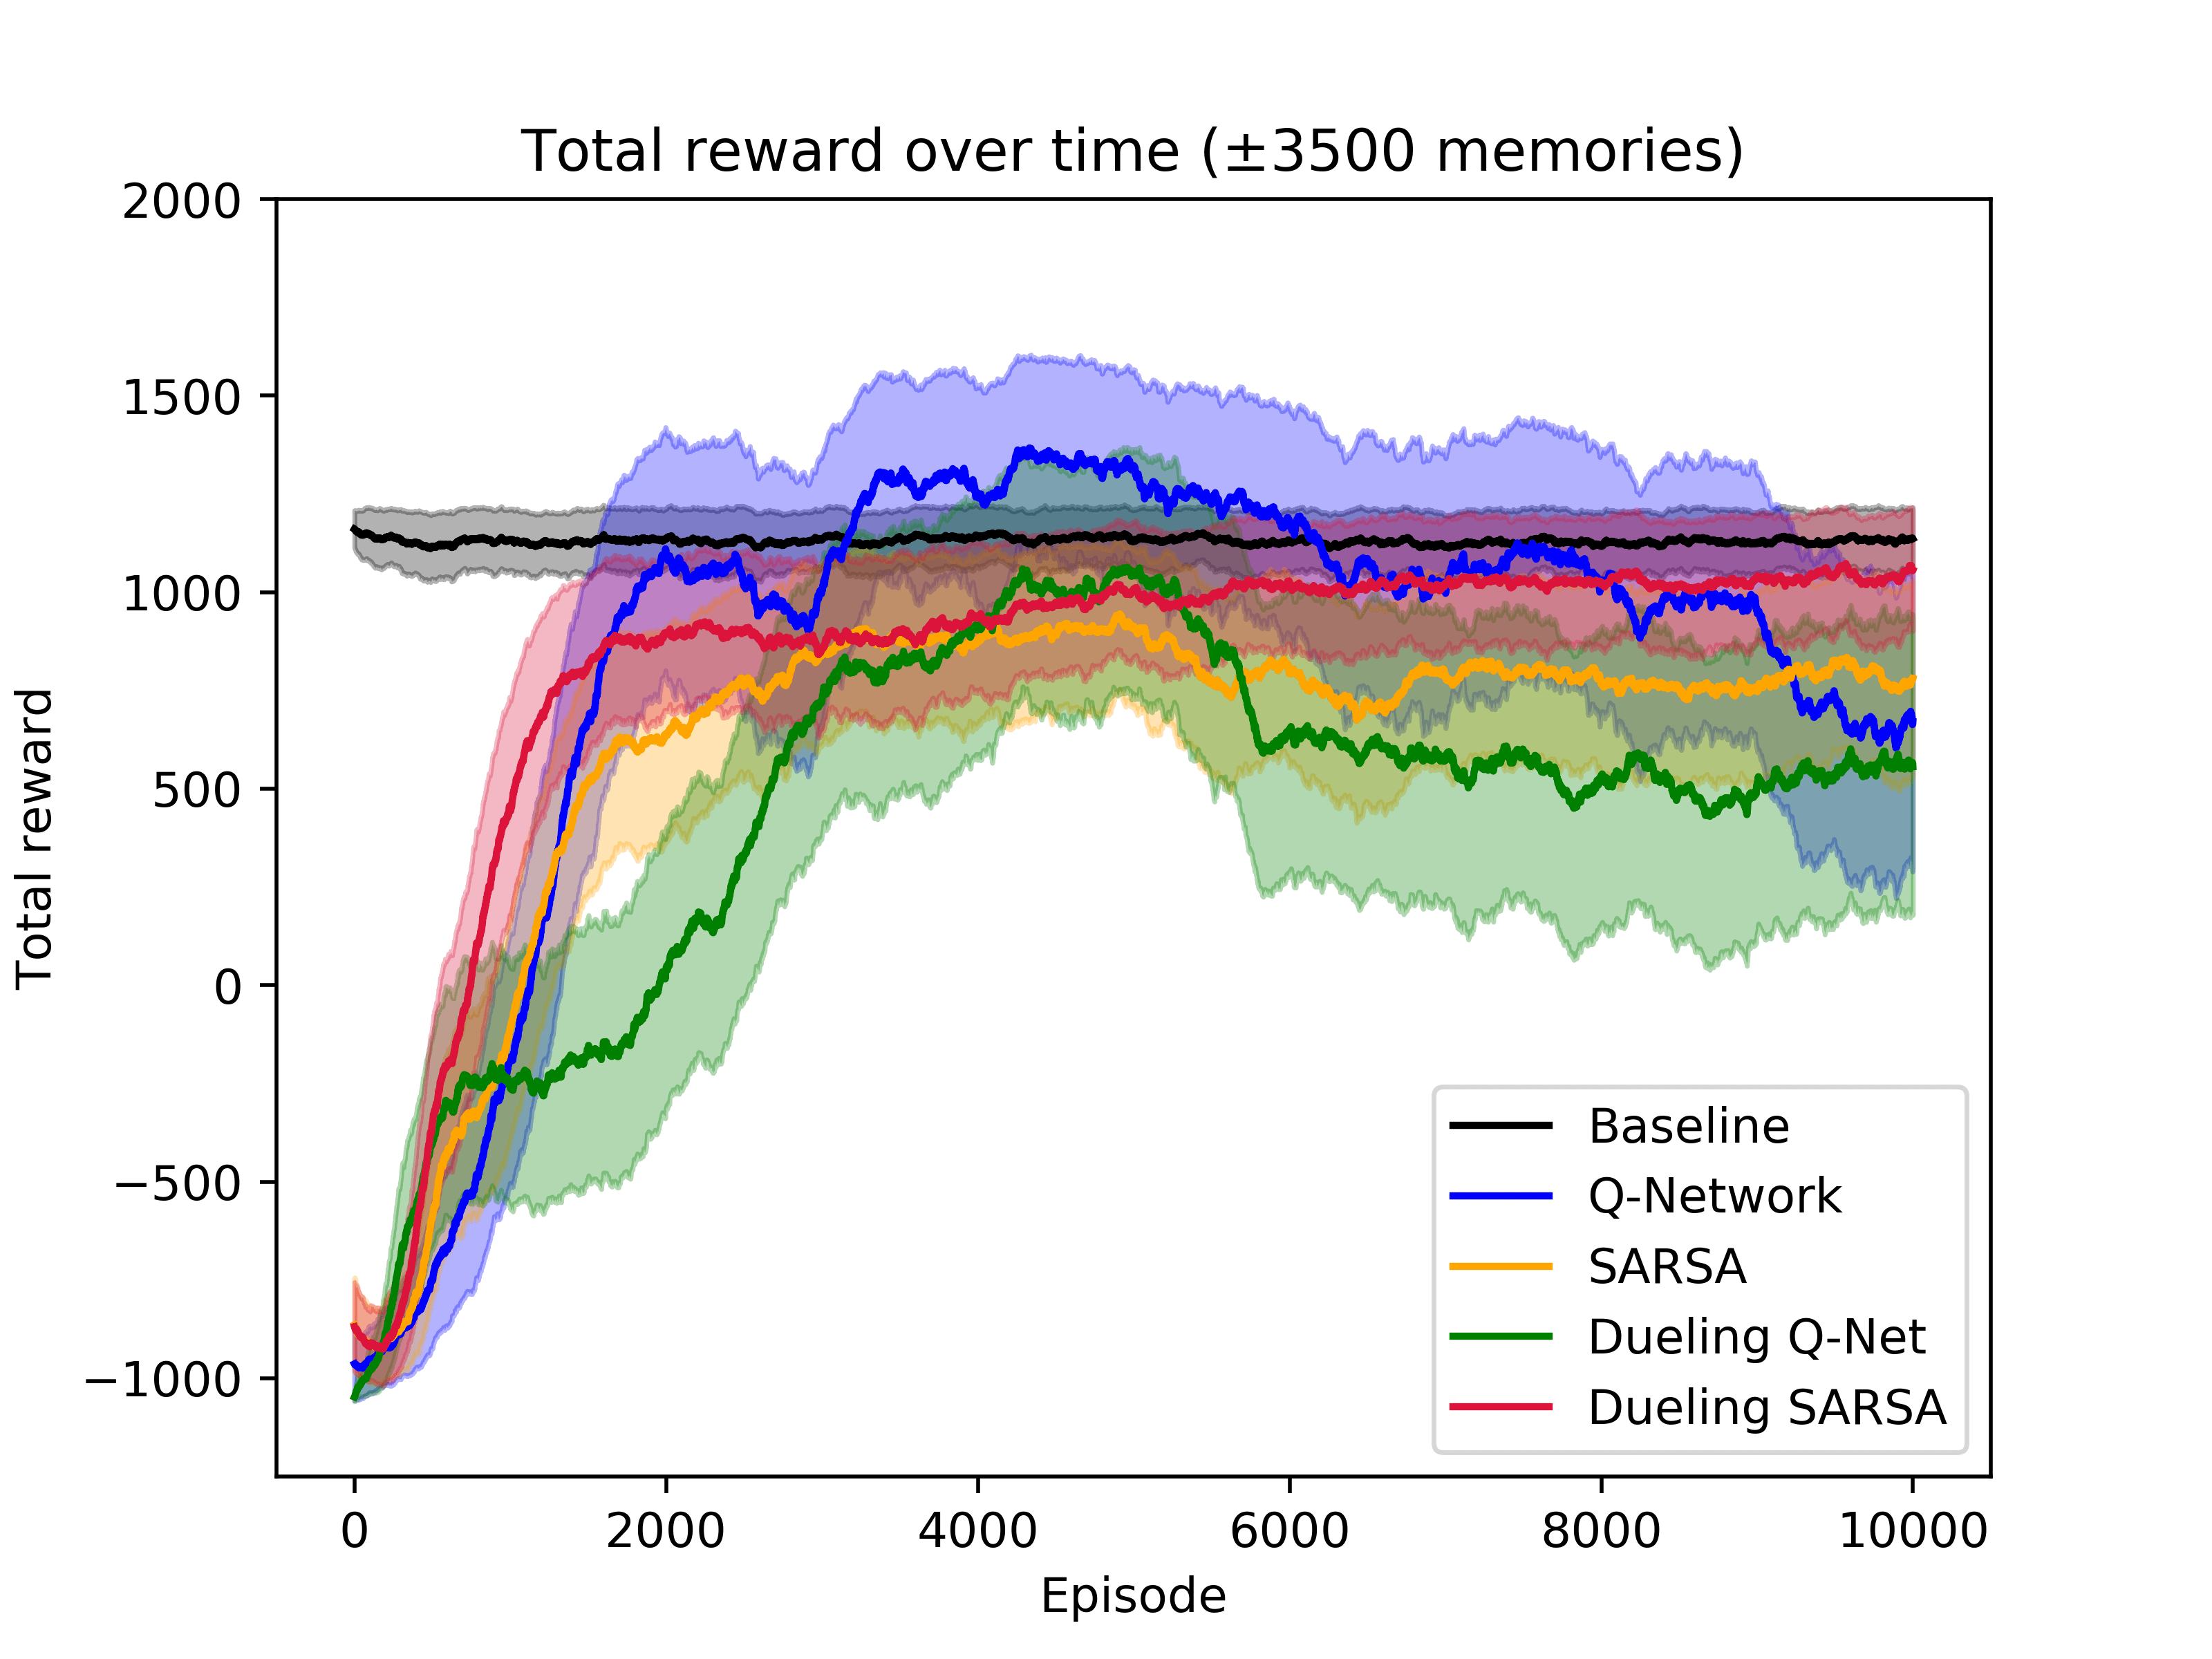
\includegraphics[width=\linewidth]{img/results/10-sized/total_rewards_100m-min.png}
    \caption{10-run averages given 100 episodes of demonstration data.}
    \label{fig:10sized-100mem}
\end{figure}
\begin{figure}[H]
    \centering
    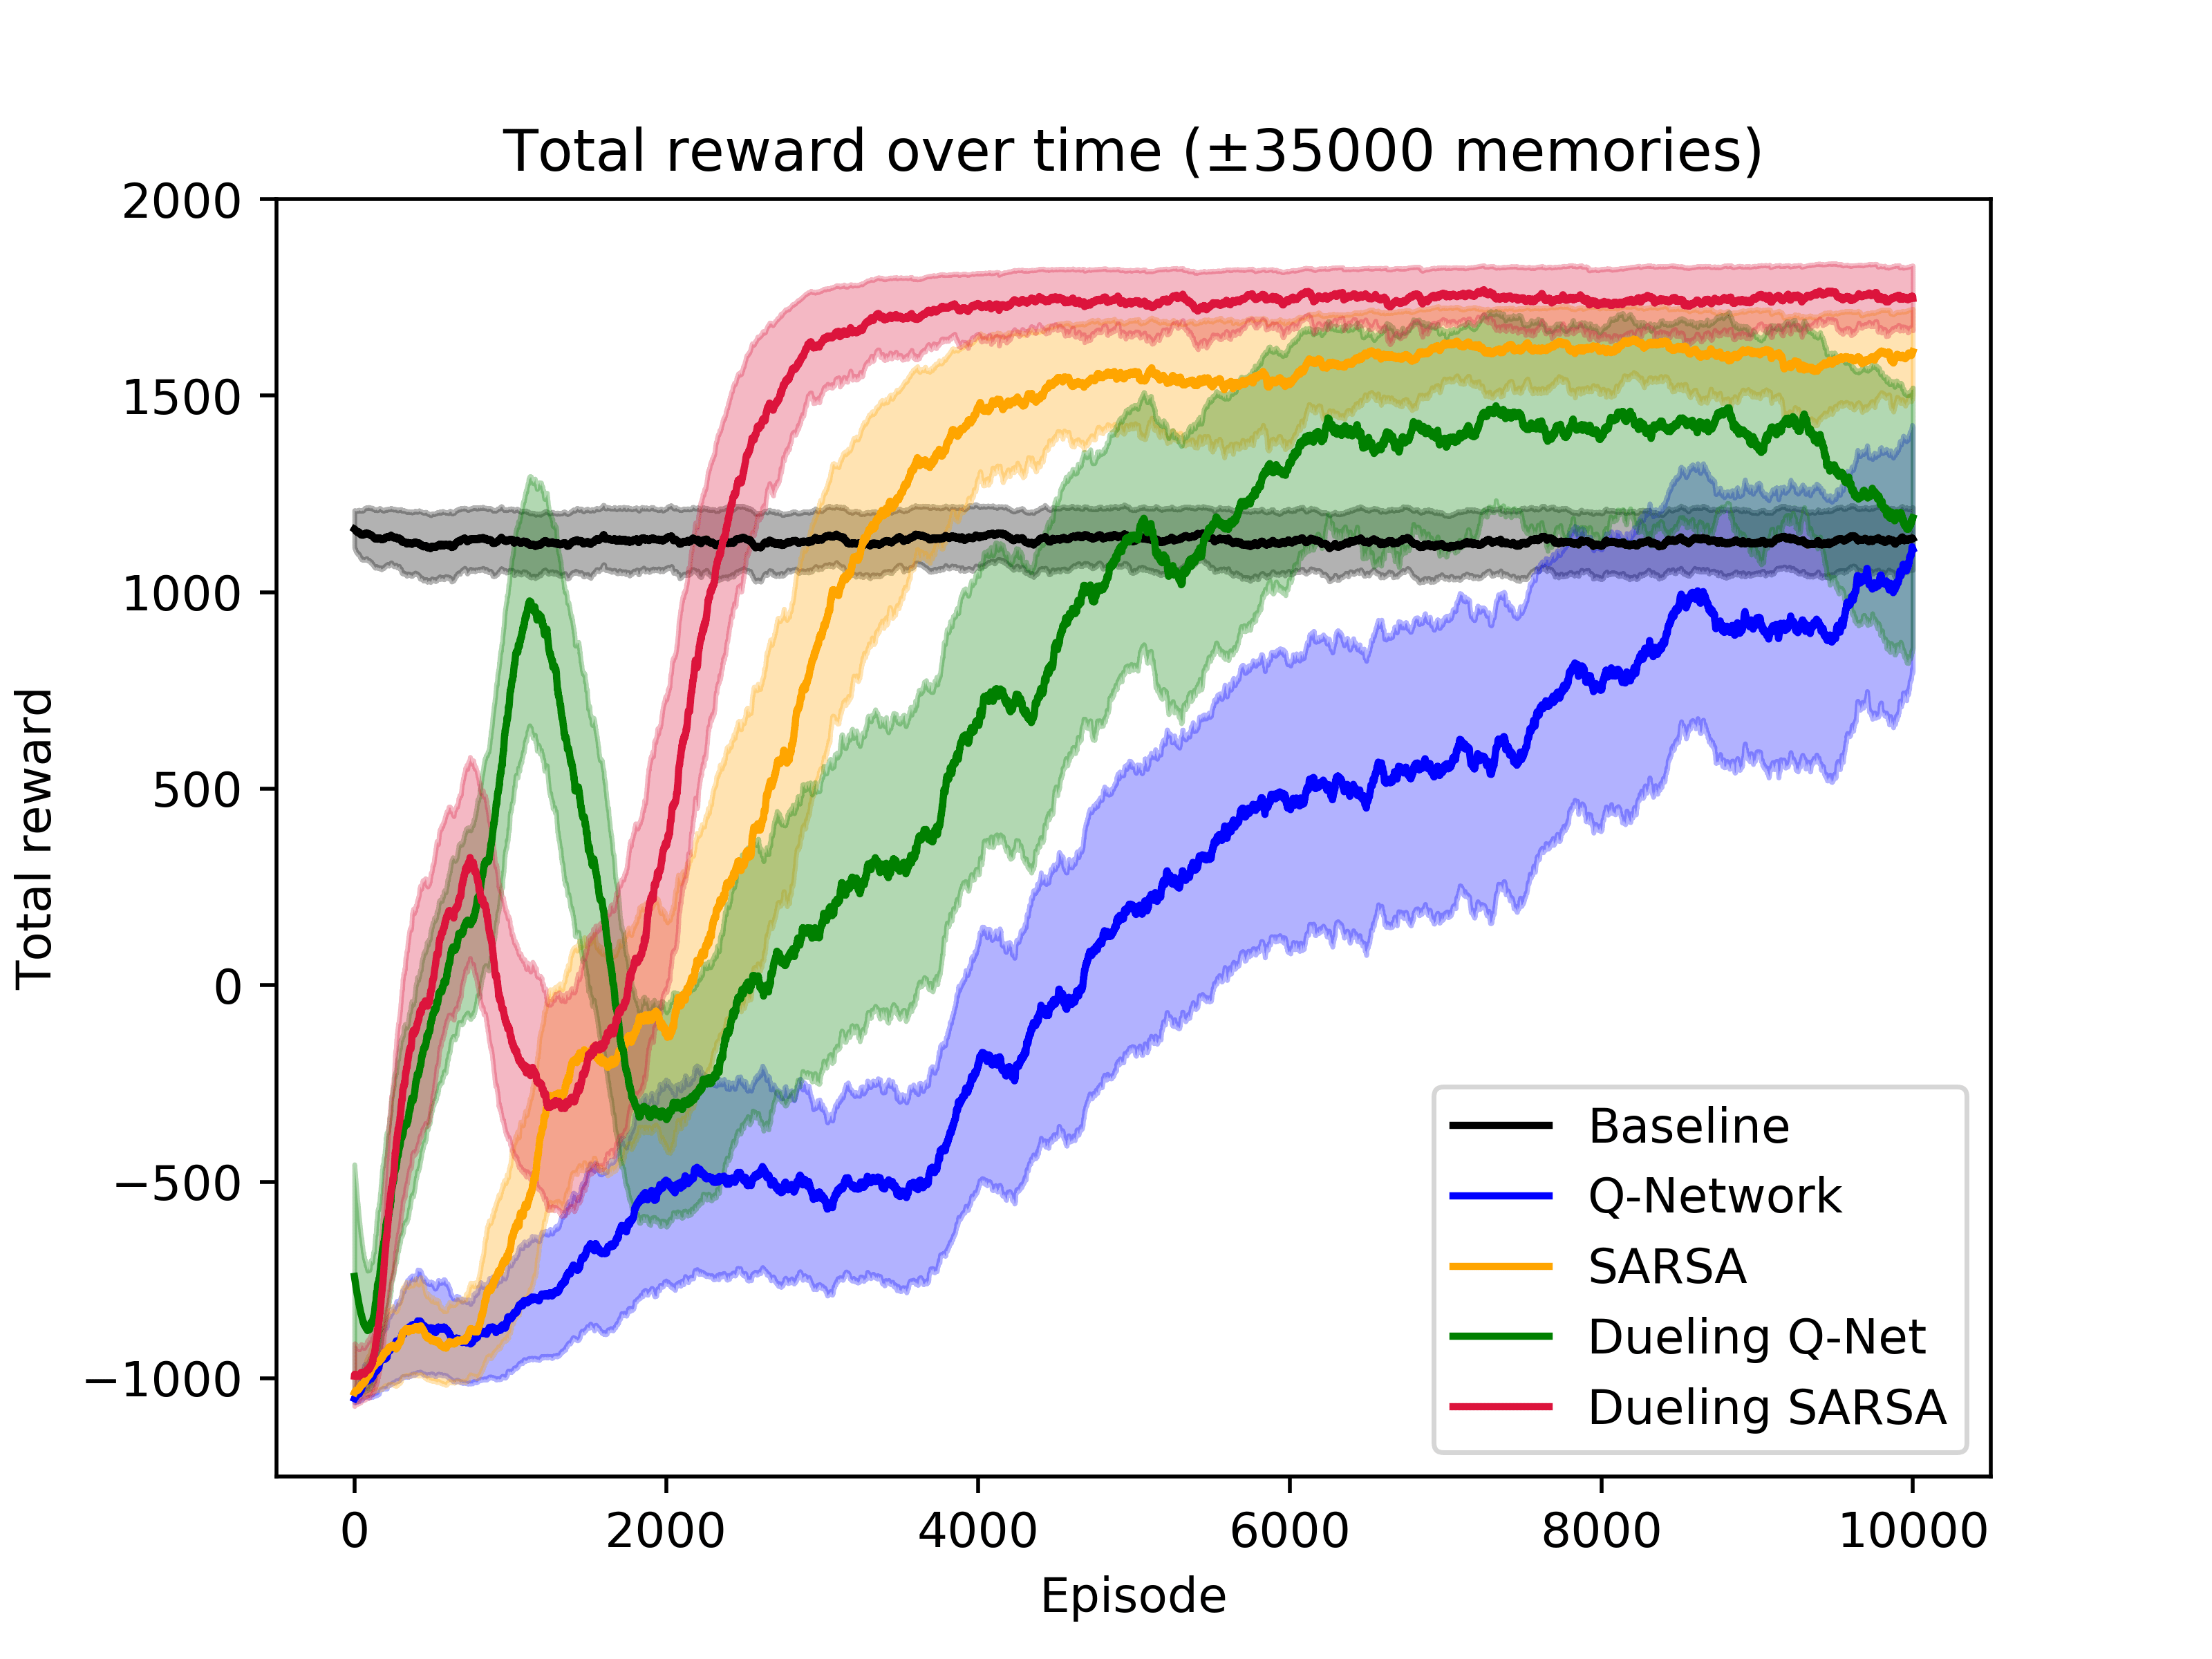
\includegraphics[width=\linewidth]{img/results/10-sized/total_rewards_1000m-min.png}
    \caption{10-run averages given 1000 episodes of demonstration data.}
    \label{fig:10sized-1000mem}
\end{figure}
% TABLES 10-sized
\begin{table}[H]
\begin{tabular}{|l|l|l|l|}
\hline
\textbf{Algorithm} & \textbf{\begin{tabular}[c]{@{}l@{}}Average\\ Reward\end{tabular}} & \textbf{\begin{tabular}[c]{@{}l@{}}Std.\\ Error\end{tabular}} & \textbf{\begin{tabular}[c]{@{}l@{}}Best\\ Reward\end{tabular}} \\ \hline
Baseline & 1129 & 1.9 & 1387 \\ \hline
Q-Network & 221 & 4.2 & 715 \\ \hline
SARSA & 132 & 3.9 & 563 \\ \hline
\begin{tabular}[c]{@{}l@{}}Dueling\\ Q-Network\end{tabular} & 956 & 4.1 & 1335 \\ \hline
\begin{tabular}[c]{@{}l@{}}Dueling\\ SARSA\end{tabular} & 241 & 2.6 & 582 \\ \hline
\end{tabular}
    \caption{Averages of the last 2500 episodes given 0 episodes of demonstation data.}
    \label{tab:10sized-0mem}
\end{table}
\begin{table}[H]
\begin{tabular}{|l|l|l|l|}
\hline
\textbf{Algorithm} & \textbf{\begin{tabular}[c]{@{}l@{}}Average\\ Reward\end{tabular}} & \textbf{\begin{tabular}[c]{@{}l@{}}Std.\\ Error\end{tabular}} & \textbf{\begin{tabular}[c]{@{}l@{}}Best\\ Reward\end{tabular}} \\ \hline
Baseline & 1129 & 1.9 & 1387 \\ \hline
Q-Network & 878 & 7.5 & 1758 \\ \hline
SARSA & 776 & 4.7 & 1292 \\ \hline
\begin{tabular}[c]{@{}l@{}}Dueling\\ Q-Network\end{tabular} & 521 & 6.8 & 1535 \\ \hline
\begin{tabular}[c]{@{}l@{}}Dueling\\ SARSA\end{tabular} & 1031 & 3.4 & 1312 \\ \hline
\end{tabular}
    \caption{Averages of the last 2500 episodes given 100 episodes of demonstation data.}
    \label{tab:10sized-100mem}
\end{table}
\begin{table}[H]
\begin{tabular}{|l|l|l|l|}
\hline
\textbf{Algorithm} & \textbf{\begin{tabular}[c]{@{}l@{}}Average\\ Reward\end{tabular}} & \textbf{\begin{tabular}[c]{@{}l@{}}Std.\\ Error\end{tabular}} & \textbf{\begin{tabular}[c]{@{}l@{}}Best\\ Reward\end{tabular}} \\ \hline
Baseline & 1129 & 1.9 & 1387 \\ \hline
Q-Network & 907 & 6.7 & 1696 \\ \hline
SARSA & 1607* & 2.8 & 1748 \\ \hline
\begin{tabular}[c]{@{}l@{}}Dueling\\ Q-Network\end{tabular} & 1369* & 5.5 & 1826 \\ \hline
\begin{tabular}[c]{@{}l@{}}Dueling\\ SARSA\end{tabular} & 1745* & 2.5 & 1860 \\ \hline
\end{tabular}
    \caption{Averages of the last 2500 episodes given 1000 episodes of demonstation data.}
    \label{tab:10sized-1000mem}
\end{table}
%FORMER 10-sized RESULTS
In Figures \ref{fig:10sized-0mem}, \ref{fig:10sized-100mem} and \ref{fig:10sized-1000mem} we see the three cases where the simulation consists of a grid of 10-by-10 cells and the algorithms are given 0, 100 or 1000 episodes of demonstration data respectively.

Firstly, in Figure \ref{fig:10sized-0mem} we see that all algorithms struggle to beat the baseline algorithm. Only the Dueling Q-Networks is able to come near. It offers a greatly increased learning speed and is able to sustain a higher maximum performance level. The other three algorithm perform similarly to each other, but noticeable worse than Dueling Q-Networks.

Secondly, in Figure \ref{fig:10sized-100mem} we see the performance of all algorithms come together. The Dueling Q-Networks which performed better than the others before, has now lost its edge and is now the worst performer. The performance of Q-Networks greatly increases when given $\pm 3500$ memories compared to none. It surpasses the baseline algorithm temporarily. SARSA and Dueling SARSA do not stand out, but also increased their performances given more memories than before.

Lastly, in Figure \ref{fig:10sized-1000mem} we see each algorithm perform differently. The Q-Network loses performance compared to the previous configuration, but still performs better than when no memories were given. The Dueling Q-Network did not improve its performance with $\pm 35000$ memories and shows a peculiar peak near the 1000th episode. SARSA has increased its performance once again and now beats the baseline algorithm. The same holds for Dueling SARSA which outperforms SARSA. Dueling SARSA shows the same, yet smaller, peak like Dueling Q-Networks. The two algorithms incorporating SARSA offer a noticeably lower standard error.

%FORMER 10-sized DISCUSSION
The results show that all algorithms perform at least reasonably well and respond very differently and sometimes uniquely to the demonstration data given at the start of the training process. Q-Networks performed best with 100 episodes of memories while the performance of Dueling Q-Networks was less dependent on the memories. The latter also showed to have a large spike in performance near the 1000th episode. This is probably due to the large amount of memories it was given. In this way, the algorithm has very few chances to make mistakes and learn from those transitions during its exploration phase. It focuses too much on the demonstrated behaviour and is hindered in trying out actions to explore consequences. This explanation can also hold for why the Q-Network performs worse with 1000 episodes of memories.
% re-read the email he sent, try to understand what he meant about the peak

SARSA showed to be one of the most consistent and trustworthy algorithms in terms of its response to the memories. In essence, more memories meant a higher sustained performance level. However, the speed at which it learned was decreased. This may also be due to the same reason mentioned; large amounts of memories hinder the algorithms exploration abilities. More memories also showed to have another positive effect on SARSA, namely its standard error. Higher performance levels came with lower standard errors. The general stability of SARSA compared to Q-Learning can be explained, as mentioned in Section \ref{sec:ql_sarsa}, by the fact that, because it is an on-policy algorithm, we effectively remove one of the three elements of the deadly triad. 

We found that combining Dueling Q-Networks and SARSA into Dueling SARSA resulted in the overall best performer, especially in high memory scenarios. It inherits the best of both worlds; the learning speed from the former, and the performance and consistency from the latter. The algorithm also inherited the performance peak from the Dueling Q-Networks, albeit not as high and slightly earlier. We estimate the maximum possible reward for an algorithm to achieve to be $\pm$1850, since it varies due to the random starting position of the agent. In Table \ref{tab:10sized-1000mem}, we see the algorithms has no problem achieving that maximum reward and having a average reward close to it. Moreover, its standard error there is similar to the baseline algorithm, which is impressive since the baseline is a hard-coded solution.

Tables \ref{tab:10sized-0mem} through \ref{tab:10sized-1000mem} show us that out of the 12 scenarios, only three times an algorithm was able to achieve an average reward higher than the baseline. All three occurred in the setting where 1000 episodes of memories were given. The Q-Network stands out as being the only one with an average reward lower than the baseline.




\subsection{14-by-14 simulations}
% FIGURES 14-sized
\begin{figure}[H]
    \centering
    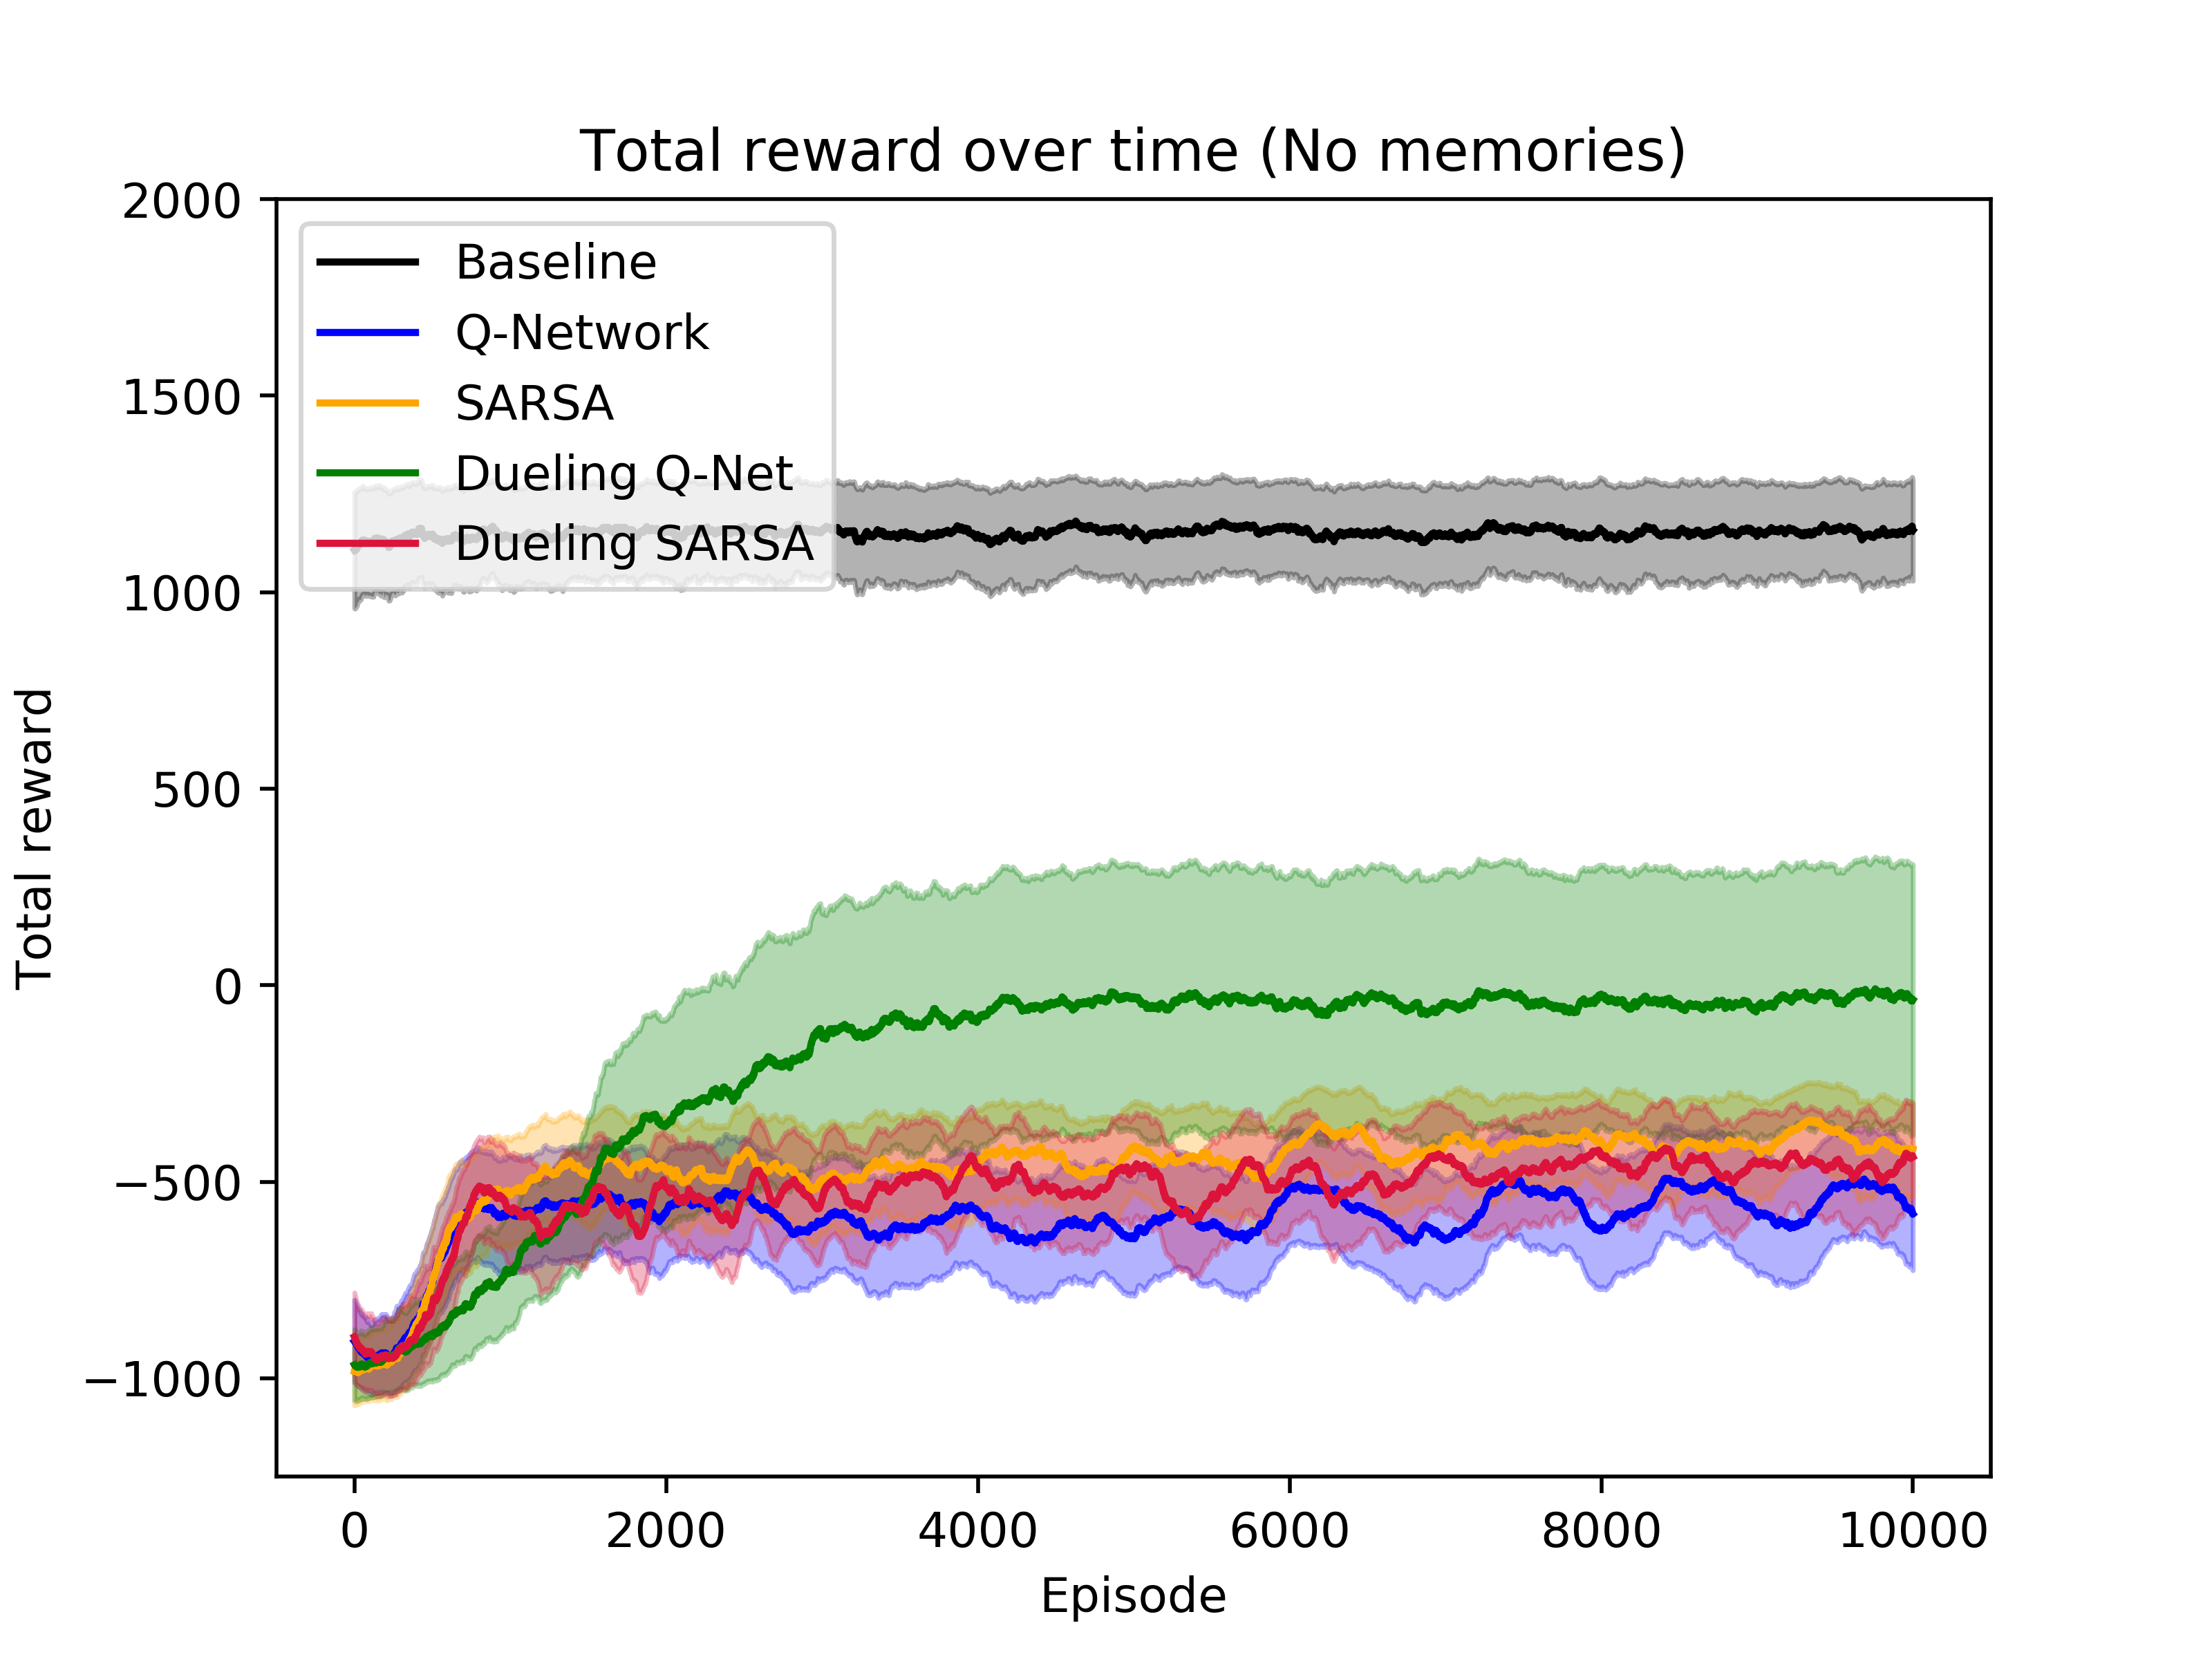
\includegraphics[width=\linewidth]{img/results/14-sized/total_rewards_0m-min.png}
    \caption{10-run averages given 0 episodes of demonstration data.}
    \label{fig:14sized-0mem}
\end{figure}
\begin{figure}[H]
    \centering
    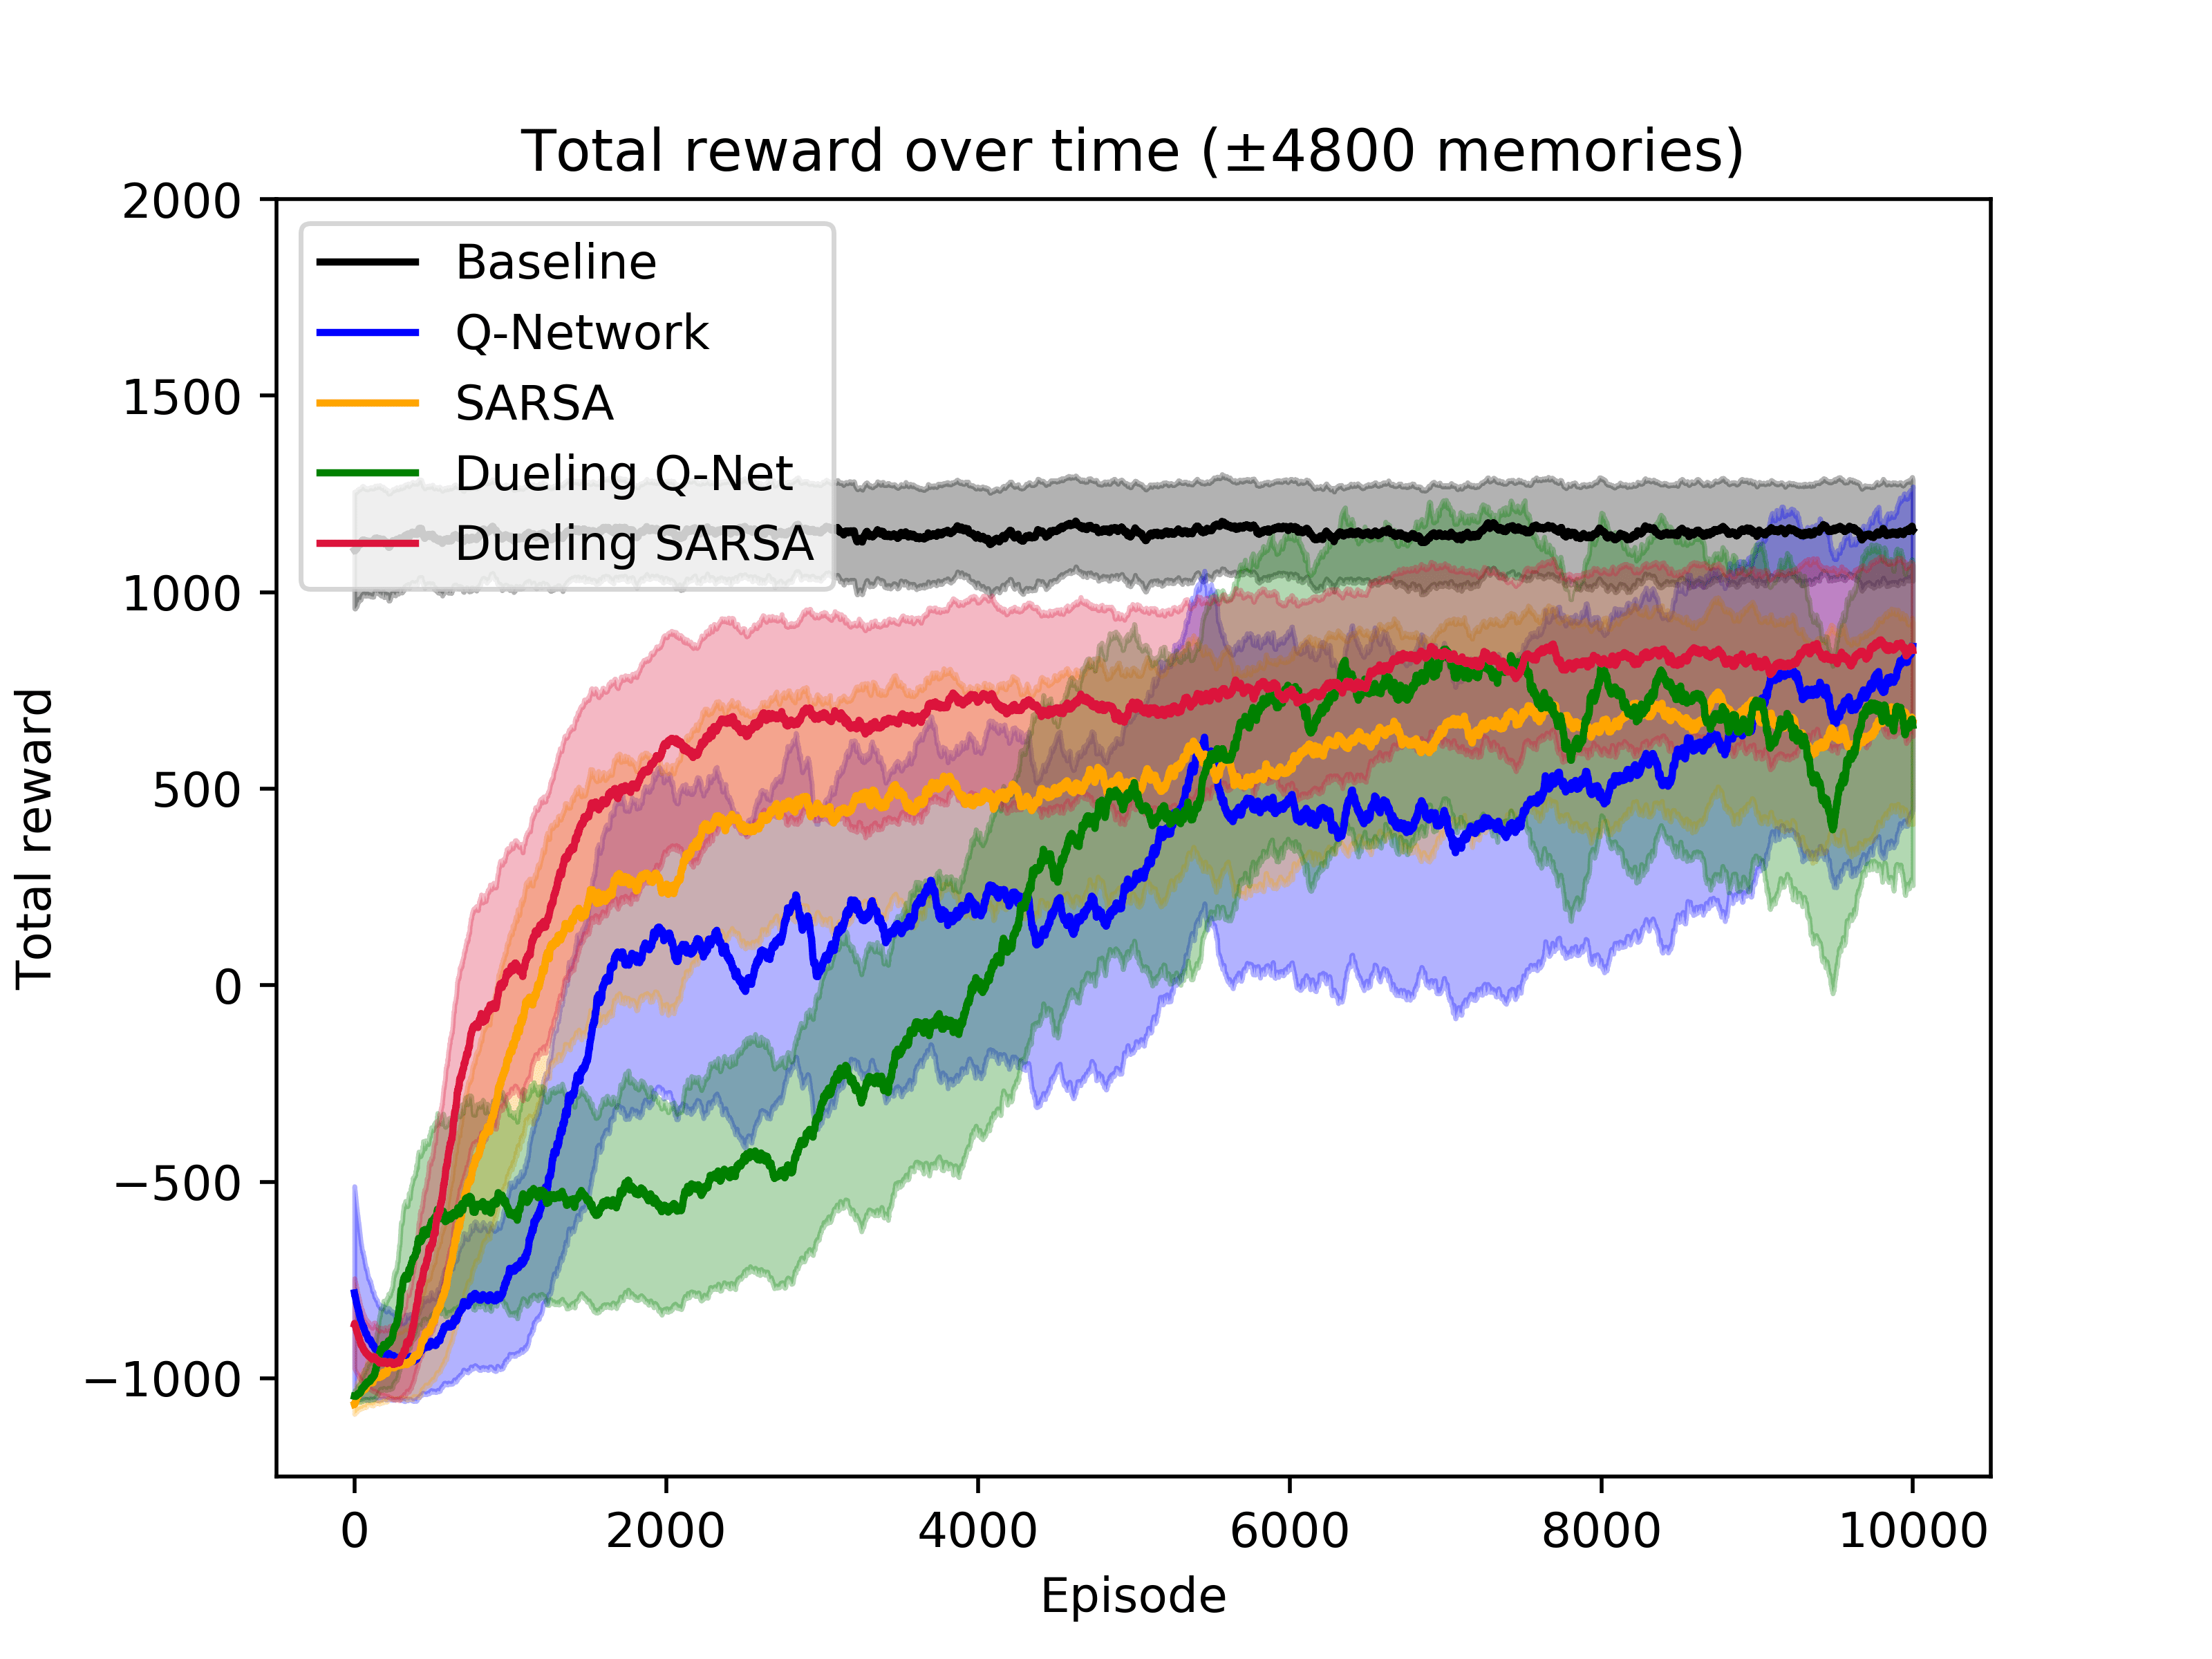
\includegraphics[width=\linewidth]{img/results/14-sized/total_rewards_100m-min.png}
    \caption{10-run averages given 100 episodes of demonstration data.}
    \label{fig:14sized-100mem}
\end{figure}
\begin{figure}[H]
    \centering
    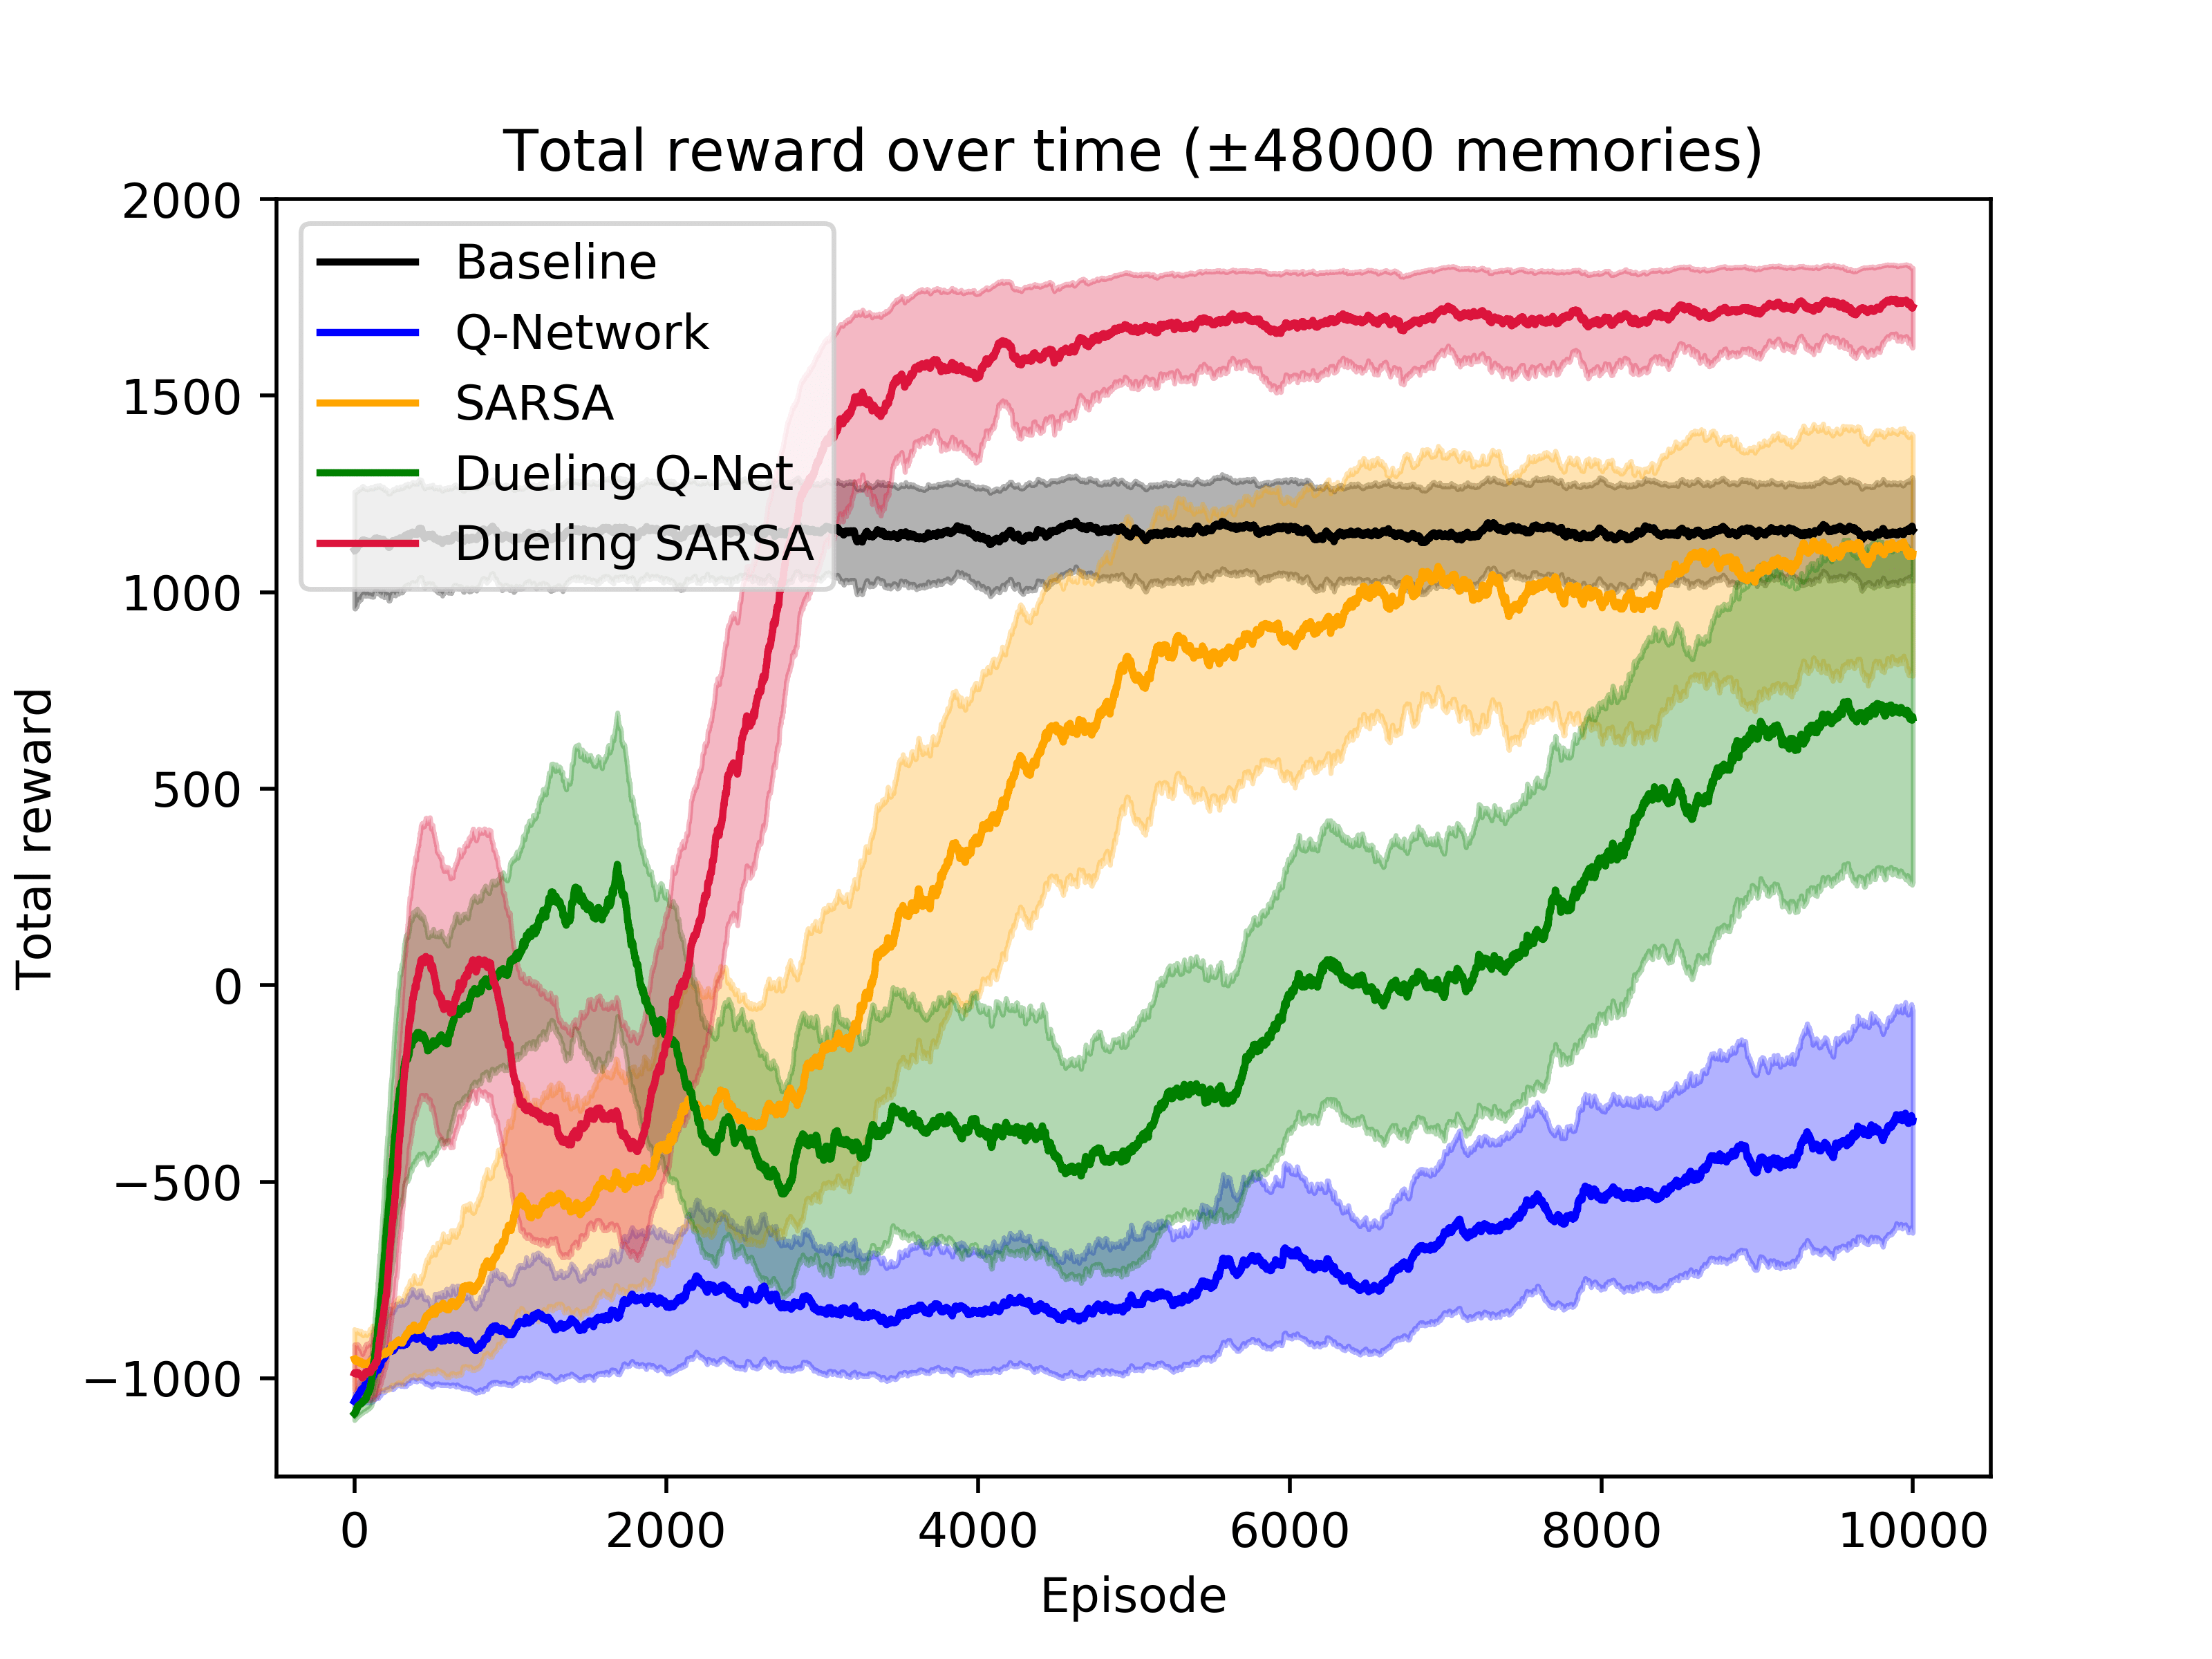
\includegraphics[width=\linewidth]{img/results/14-sized/total_rewards_1000m-min.png}
    \caption{10-run averages given 1000 episodes of demonstration data.}
    \label{fig:14sized-1000mem}
\end{figure}
% TABLES 14-sized
\begin{table}[H]
\begin{tabular}{|l|l|l|l|}
\hline
\textbf{Algorithm} & \textbf{\begin{tabular}[c]{@{}l@{}}Average\\ Reward\end{tabular}} & \textbf{\begin{tabular}[c]{@{}l@{}}Std.\\ Error\end{tabular}} & \textbf{\begin{tabular}[c]{@{}l@{}}Best\\ Reward\end{tabular}} \\ \hline
Baseline & 1152 & 2.8 & 1513 \\ \hline
Q-Network & -550 & 2.9 & -139 \\ \hline
SARSA & -398 & 2.4 & -92 \\ \hline
\begin{tabular}[c]{@{}l@{}}Dueling\\ Q-Network\end{tabular} & -40 & 3.0 & 349 \\ \hline
\begin{tabular}[c]{@{}l@{}}Dueling\\ SARSA\end{tabular} & -455 & 2.6 & -44 \\ \hline
\end{tabular}
    \caption{Averages of the last 2500 episodes given 0 episodes of demonstation data.}
    \label{tab:14sized-0mem}
\end{table}
\begin{table}[H]
\begin{tabular}{|l|l|l|l|}
\hline
\textbf{Algorithm} & \textbf{\begin{tabular}[c]{@{}l@{}}Average\\ Reward\end{tabular}} & \textbf{\begin{tabular}[c]{@{}l@{}}Std.\\ Error\end{tabular}} & \textbf{\begin{tabular}[c]{@{}l@{}}Best\\ Reward\end{tabular}} \\ \hline
Baseline & 1152 & 2.8 & 1513 \\ \hline
Q-Network & 652 & 7.0 & 169 \\ \hline
SARSA & 670 & 5.3 & 1275 \\ \hline
\begin{tabular}[c]{@{}l@{}}Dueling\\ Q-Network\end{tabular} & 667 & 7.8 & 1748 \\ \hline
\begin{tabular}[c]{@{}l@{}}Dueling\\ SARSA\end{tabular} & 836 & 4.1 & 1249 \\ \hline
\end{tabular}
    \caption{Averages of the last 2500 episodes given 100 episodes of demonstation data.}
    \label{tab:14sized-100mem}
\end{table}
\begin{table}[H]
\begin{tabular}{|l|l|l|l|}
\hline
\textbf{Algorithm} & \textbf{\begin{tabular}[c]{@{}l@{}}Average\\ Reward\end{tabular}} & \textbf{\begin{tabular}[c]{@{}l@{}}Std.\\ Error\end{tabular}} & \textbf{\begin{tabular}[c]{@{}l@{}}Best\\ Reward\end{tabular}} \\ \hline
Baseline & 1152 & 2.8 & 1513 \\ \hline
Q-Network & -459 & 5.0 & 411 \\ \hline
SARSA & 1057 & 5.6 & 1626 \\ \hline
\begin{tabular}[c]{@{}l@{}}Dueling\\ Q-Network\end{tabular} & 522 & 7.7 & 1534 \\ \hline
\begin{tabular}[c]{@{}l@{}}Dueling\\ SARSA\end{tabular} & 1713* & 3.0 & 1846 \\ \hline
\end{tabular}
    \caption{Averages of the last 2500 episodes given 1000 episodes of demonstation data.}
    \label{tab:14sized-1000mem}
\end{table}
%FORMER 14-sized RESULTS
In Figure \ref{fig:14sized-0mem}, \ref{fig:14sized-100mem} and \ref{fig:14sized-1000mem} we see the three cases where the simulation has a grid size of 14-by-14 and the algorithms are given 0, 100 or 1000 episodes of demonstation data.

Firstly, in Figure \ref{fig:14sized-0mem} we see results comparable to Figure \ref{fig:10sized-0mem}, however the performance difference of Dueling Q-Networks compared to the rest has decreased. The best performing algorithm here does not come close to the performance of the baseline.

Secondly, in Figure \ref{fig:14sized-100mem} we see results similar to Figure \ref{fig:10sized-100mem}, but no algorithm is able to beat the baseline like Q-Networks was able to before.

Lastly, in Figure \ref{fig:14sized-1000mem} we once again see results comparable to Figure \ref{fig:10sized-1000mem}, however only Dueling SARSA is now able to beat the baseline algorithm. SARSA is able to perform at the same level as the baseline in the end. The (Dueling) Q-Networks do not offer good performance, but Dueling Q-Networks does outperform Q-Networks.

%FORMER 14-sized DISCUSSION
When switching to a simulation consisting of a square grid of size 14 instead of 10, we see the algorithms struggle a lot more in general. Since we use vision grids, this nearly doubles the amount of inputs from 300 to 588. The relatively small hidden layer used seems to struggle to properly learn and process all information. The number of episodes that the algorithm was allowed to learn for was also kept constant which could explain the low overall performances.

When the algorithms are not given any memories the Dueling Q-Networks is still able to perform better than the rest, but it achieves similar scores to the worst performers in the 10-by-10 simulation. Q-Networks, SARSA and Dueling SARSA seem to barely improve at all. When given 100 or 1000 episodes of memories the Dueling Q-Network improves in both cases, but does not achieve the same levels of performance. The Q-Network shows the same behaviour as before as it performs best with the medium amount of memories given and drops that advantage when given a high amount. This algorithm is also not able to solve the problem. Both Q-Network and Dueling Q-Networks fail to solve the problem and beat the baseline in all cases.

SARSA is still very receptive to memories with its best performance being the scenario where $\pm 48000$ memories were given. Here it is the only algorithm so far that is able to match the baseline algorithm. The only algorithm that is able to consistently beat it is Dueling SARSA in the high memory scenario. It shows performance very similar to the 10-by-10 simulation. The only difference is that it tops out later and suffers from a slightly higher standard error.

One other interesting thing to mention is that in the 14-by-14 simulation Both Dueling Q-Networks and Dueling SARSA show a peak in performance at the start of the learning process as well. While the peak is now not as high, both algorithms have a peak of roughly the same size. The peaks are more spread out and Dueling SARSA's peak still happens earlier. In the 10-by-10 simulation both algorithms managed to quickly regain performance and continue learning after this peak, while in the 14-by-14 simulation only Dueling SARSA is able to continue learning properly.

To conclude this section, we can look at the figures with an asterisk (*) in Tables \ref{tab:10sized-0mem} through \ref{tab:14sized-1000mem}. These are the cases where the average score of the last 2500 episodes of an algorithm was greater than the same average of the baseline. In the 24 algorithm/memory/size combinations, this happened only four times. Two of which were performed by the Dueling SARSA algorithm. With the highest amount of memories it was the only algorithm to solve the task successfully on both the 10-by-10 and 14-by-14 simulations. When looking at just the scenario where the algorithms were given the maximum amount of memories on a 10-by-10 simulation, two other algorithms were able to succeed: Dueling Q-Networks and SARSA. This rhymes nicely with the expectation that combining these two algorithms into Dueling SARSA makes it inherit the best of both worlds.
%!TEX root = report.tex

\section{Discussion}\label{sec:discussion}
The results show that all algorithms perform at least reasonably well (with the exception of some larger map sizes) and respond very differently and sometimes uniquely to the demonstration data given at the start of the training process. 

Starting with the 10-by-10 sized simulation (see Figures \ref{fig:10sized-nomem}, \ref{fig:10sized-100mem} and \ref{fig:10sized-1000mem}), Q-Networks performed best with 100 episodes of memories while the performance of Dueling Q-Networks was less dependent on the memories. The latter also showed to have a large spike in performance near the 1000th episode. This can be due to the memory buffer being filled completely by demonstration data. Because of this, the algorithm has very few chances to make mistakes and learn from those transitions during its exploration phase. It focuses too much on the demonstrated behaviour and is hindered in trying out actions to explore consequences. This explanation can also hold for why the Q-Network performs worse with 1000 episodes of memories.

SARSA showed to be one of the most consistent and trustworthy algorithms in terms of its response to the memories. In essence, more memories meant a higher sustained performance level. However, the speed at which it learned was decreased. This may also be due to the same reason mentioned; large amounts of memories hinder the algorithms exploration abilities. More memories also showed to have another positive effect on SARSA, namely its standard error. Higher performance levels came with lower standard errors. The general stability of SARSA compared to Q-Learning can be explained, as mentioned in Section \ref{sec:ql_sarsa}, by the fact that, because it is an on-policy algorithm, we effectively remove one of the three elements of the deadly triad. 

We found that combining Dueling Q-Networks and SARSA into Dueling SARSA proved to be and success and resulted in the overall best performer, especially in high memory scenarios. It inherits the best of both worlds; the learning speed from the first, and the performance and consistency from the latter. The algorithm inherited the performance peak from the Dueling Q-Networks, albeit not as high and slightly earlier. We estimate the maximum possible reward for an algorithm to achieve to be $\pm$1850. In Figure \ref{fig:10sized-1000mem} the algorithms performance gets very close to that maximum score and stays there throughout the rest of the training episodes. Moreover, its standard error there is similar to the baseline algorithm, which is impressive since the latter is a hard-coded solution.


When switching to a simulation consisting of a square grid of size 14 instead of 10 (see figures \ref{fig:14sized-nomem}, \ref{fig:14sized-100mem} and \ref{fig:14sized-1000mem}), we see the algorithms struggle a lot more in general. This setting nearly doubles the amount of inputs for relatively small neural networks, which seem to struggle to properly learn and process all information. The number of episodes that the algorithm was allowed to learn for was also kept constant which could explain the low overall performances.

When the algorithms are not given any memories the Dueling Q-Networks is still able to perform better than the rest, but it achieves similar scores to the worst performers in the 10-by-10 simulation. Q-Networks, SARSA and Dueling SARSA seem to barely improve at all. When given 100 or 1000 episodes of memories the Dueling Q-Network improves in both cases, but does not achieve the same levels of performance. The Q-Network shows the same behaviour as before as it performs best with the medium amount of memories given and drops that advantage when given a high amount. This algorithm is also not able to solve the problem. Both Q-Network and Dueling Q-Networks fail to solve the problem and beat the baseline in all cases.

SARSA is still very receptive to memories with its best performance being the scenario where $\pm 48000$ memories were given. Here it is the only algorithm so far that is able to match the baseline algorithm. The only algorithm that is able to consistently beat it is Dueling SARSA in the high memory scenario. It shows performance very similar to the 10-by-10 simulation. The only difference is that it tops out later and suffers from a slightly higher standard error.

One last interesting thing to mention is that also in the 14-by-14 simulation Both Dueling Q-Networks and Dueling SARSA show a peak in performance at the start of the learning process. While the peak is now not as high, both algorithms have a peak of roughly the same size. The peaks are more spread out and Dueling SARSA's peak still happens earlier. In the 10-by-10 simulation both algorithms managed to quickly regain performance and continue learning after this peak, while in the 14-by-14 simulation only Dueling SARSA is able to continue learning properly.

\section{Conclusion}\label{sec:conclusions}
%What went well, what can be improved, other remarks etc
The simulation environment was very simplified. We have the functionality to determine the wind speed and direction but did not have the time to explore those options. There is also support for more cell types such as grass versus trees or rivers, each with different properties for a more complex and realistic environment. We believe this should be investigated in subsequent research, because the system should ultimately prove itself reliable in more complex environments (that is real life).

The reward function is, in its current form, very hard for an agent to learn with. It provides very sparse and very delayed rewards, this can be improved to provide a more smooth gradient and allowing for faster and more stable learning, and less reliance on demonstration data. 

Since all algorithms are based on connectionist reinforcement learning, they are likely to benefit from other improvements proven to be useful. Examples we think would perform well are prioritized experience replay \citep{schaul2015prioritized} and Deep Q-Networks \citep{mnih2015human}. Using a deep network with convolutional layers might extract some meaningful information that it cannot otherwise, like shape of the circle and position of the agent relative to it for example.

The results may have shown more interesting patterns for longer runs (more than 10,000 episodes). We might have seen the same patterns in performance for the 14-by-14 maps as for the 10-by-10 ones, just on a larger scale. It also likely that some patterns are not visible even on the smaller map size with 10000 episodes, such as the drop in performance for Q-Learning without Dueling networks.


\bibliographystyle{plainnat}
\bibliography{literature}

\clearpage

\begin{appendices}
    \section{Appendix}\label{ap:appendix}
% PLOTS
\begin{figure}[H]
    \centering
    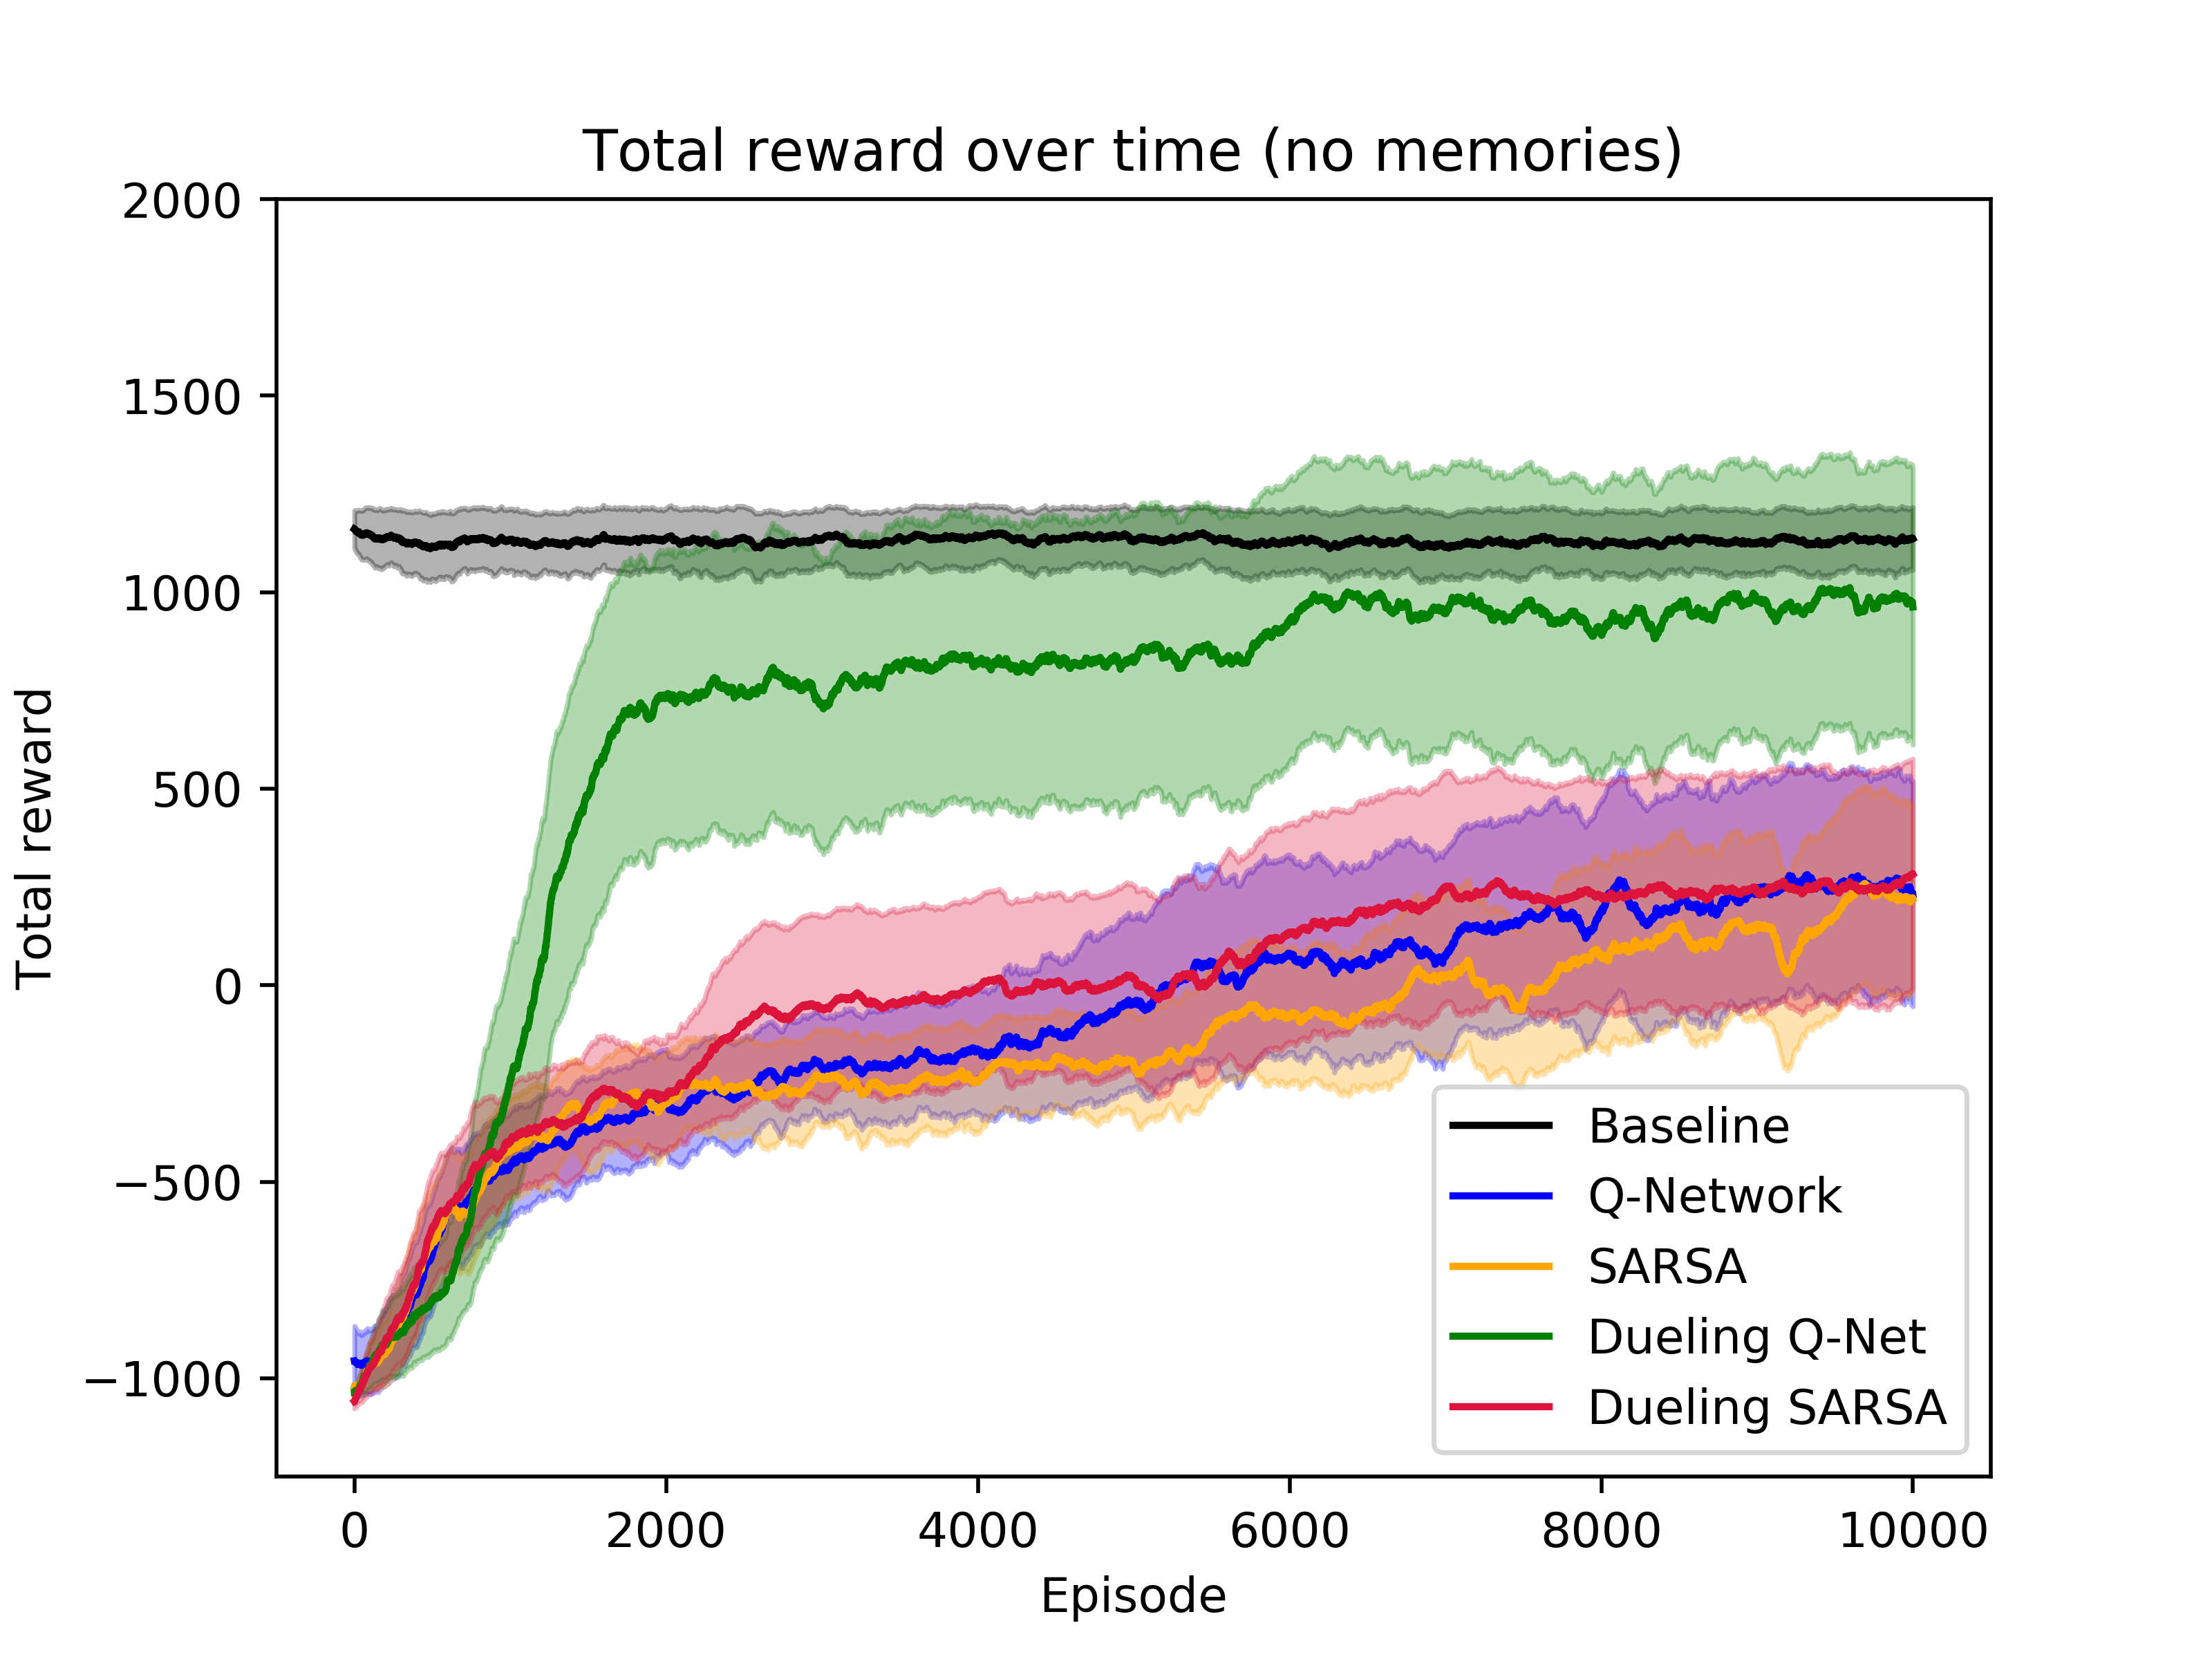
\includegraphics[width=\linewidth]{img/results/10-sized/total_rewards_0m-min.png}
    \caption{10-by-10 grid given no demonstation data.}
    \label{fig:10sized-nomem}
    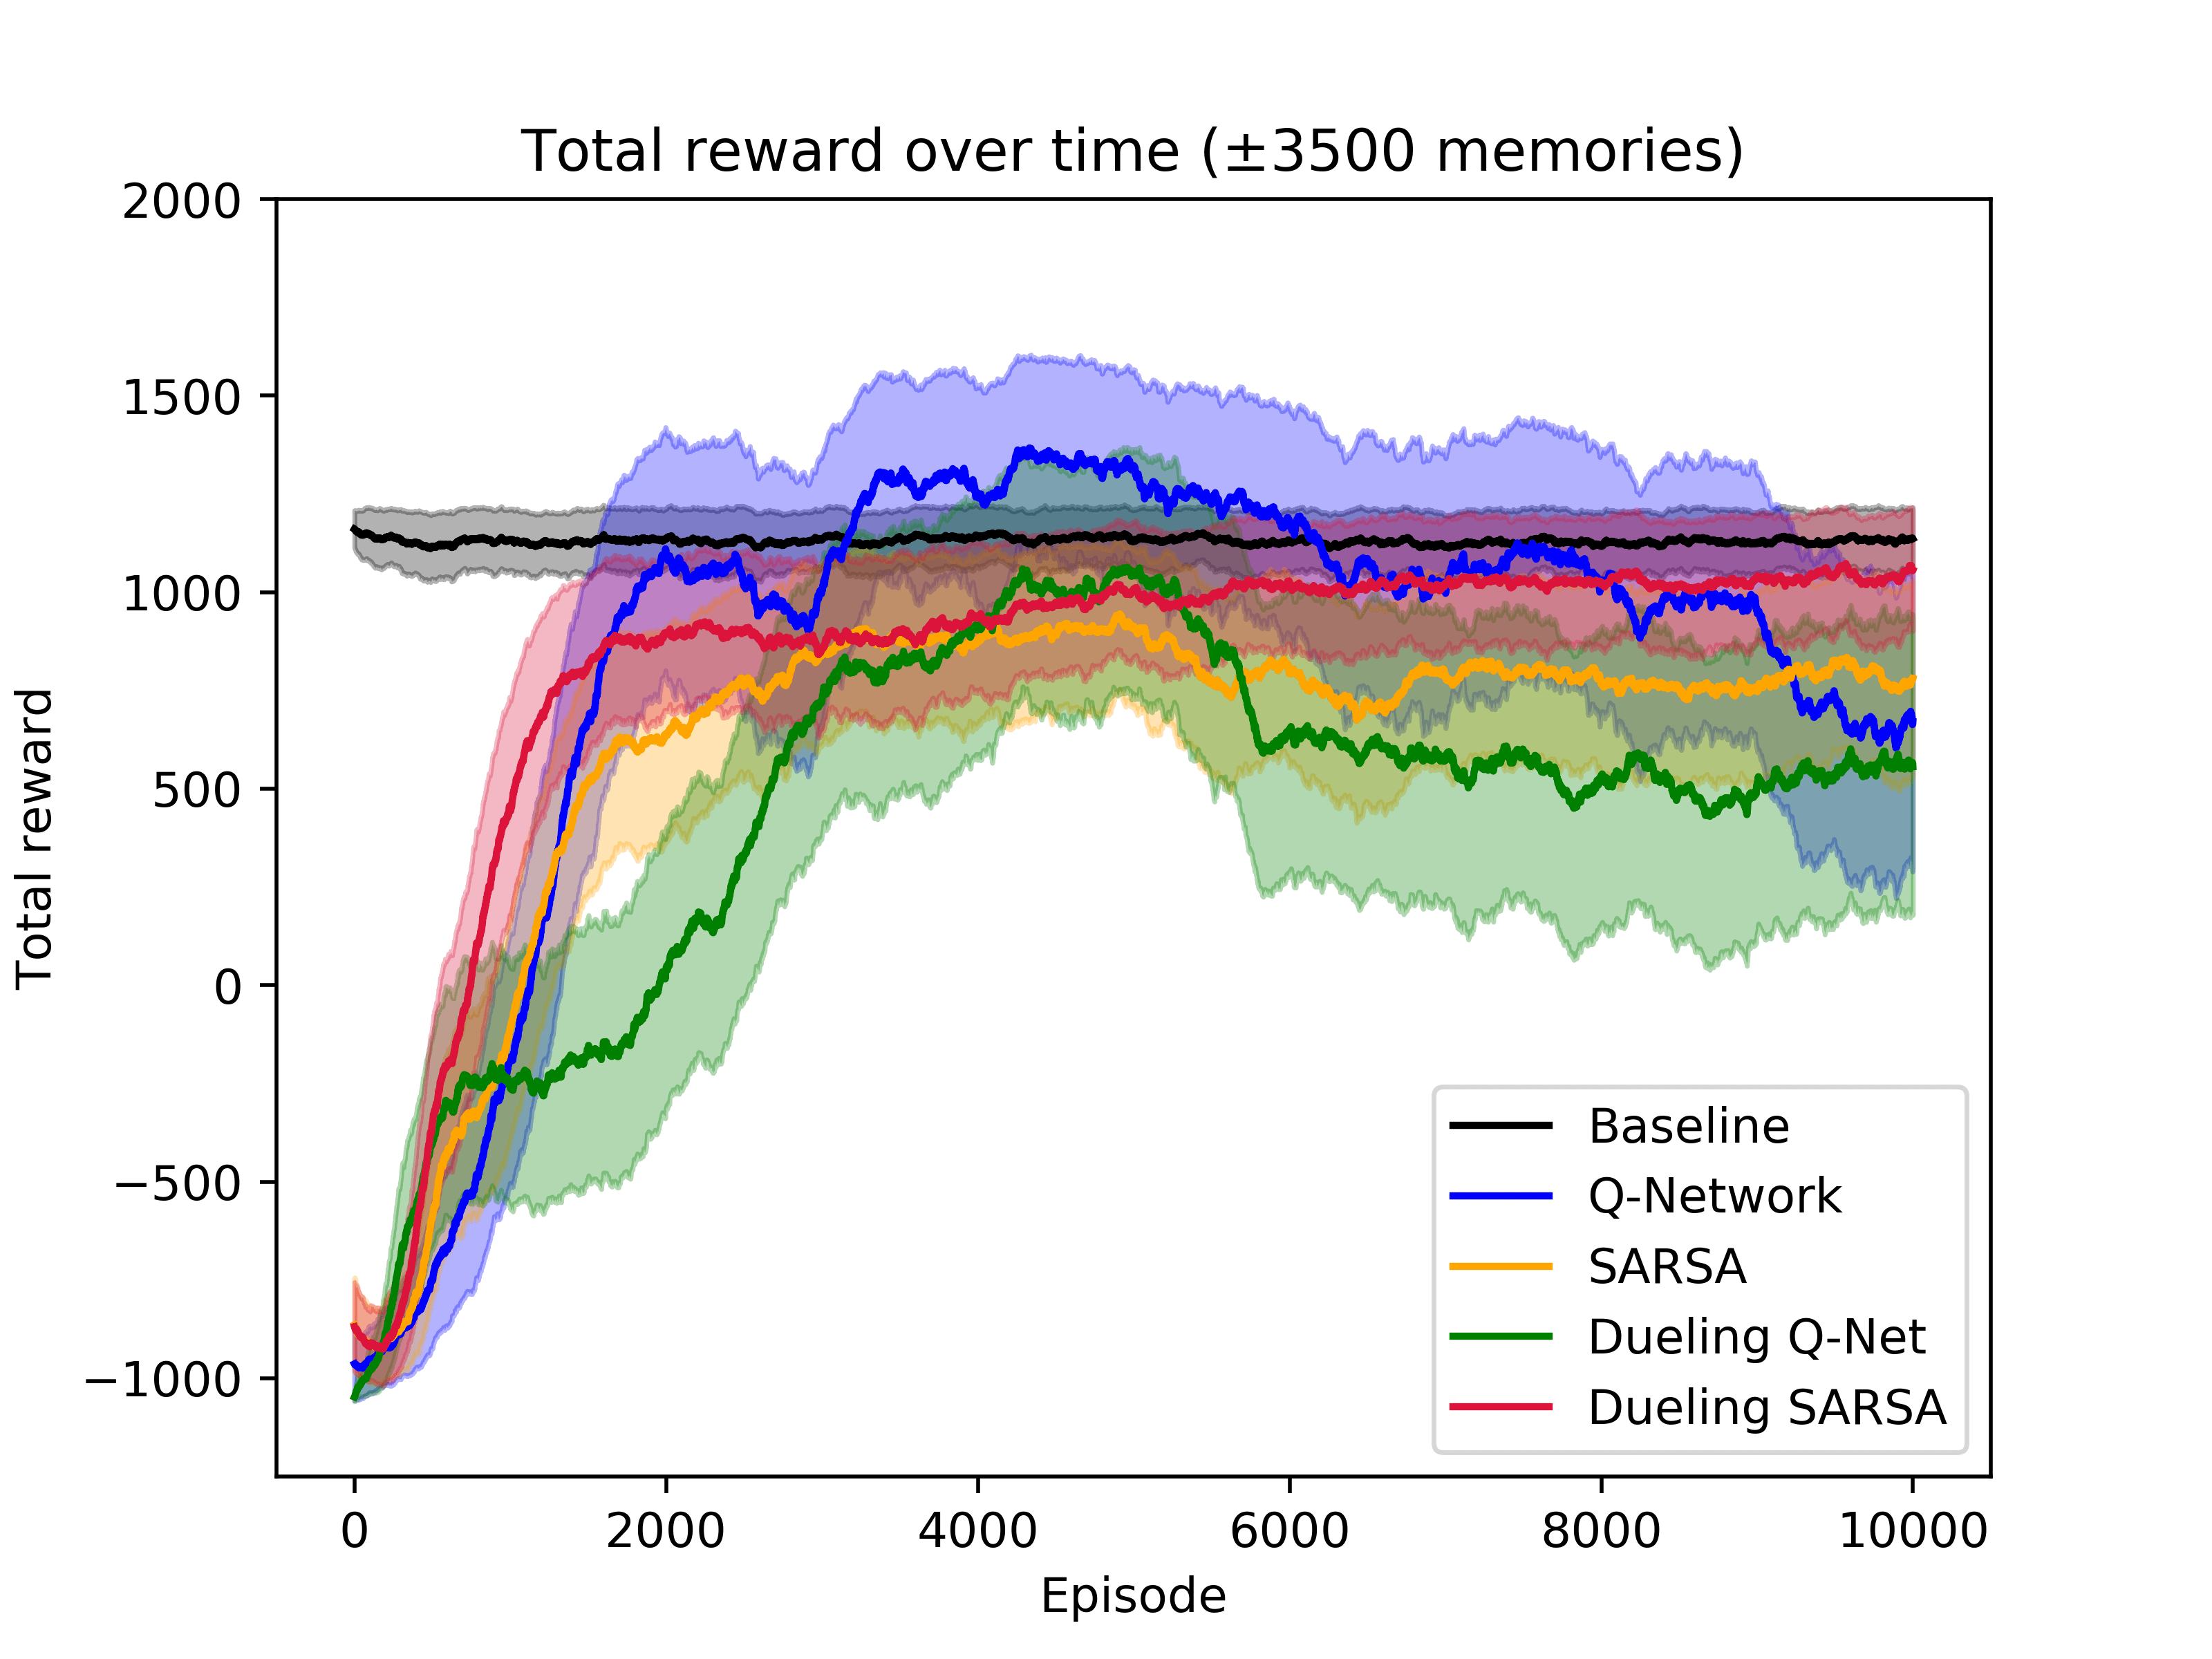
\includegraphics[width=\linewidth]{img/results/10-sized/total_rewards_100m-min.png}
    \caption{10-by-10 grid given 100 episodes of demonstation data.}
    \label{fig:10sized-100mem}
    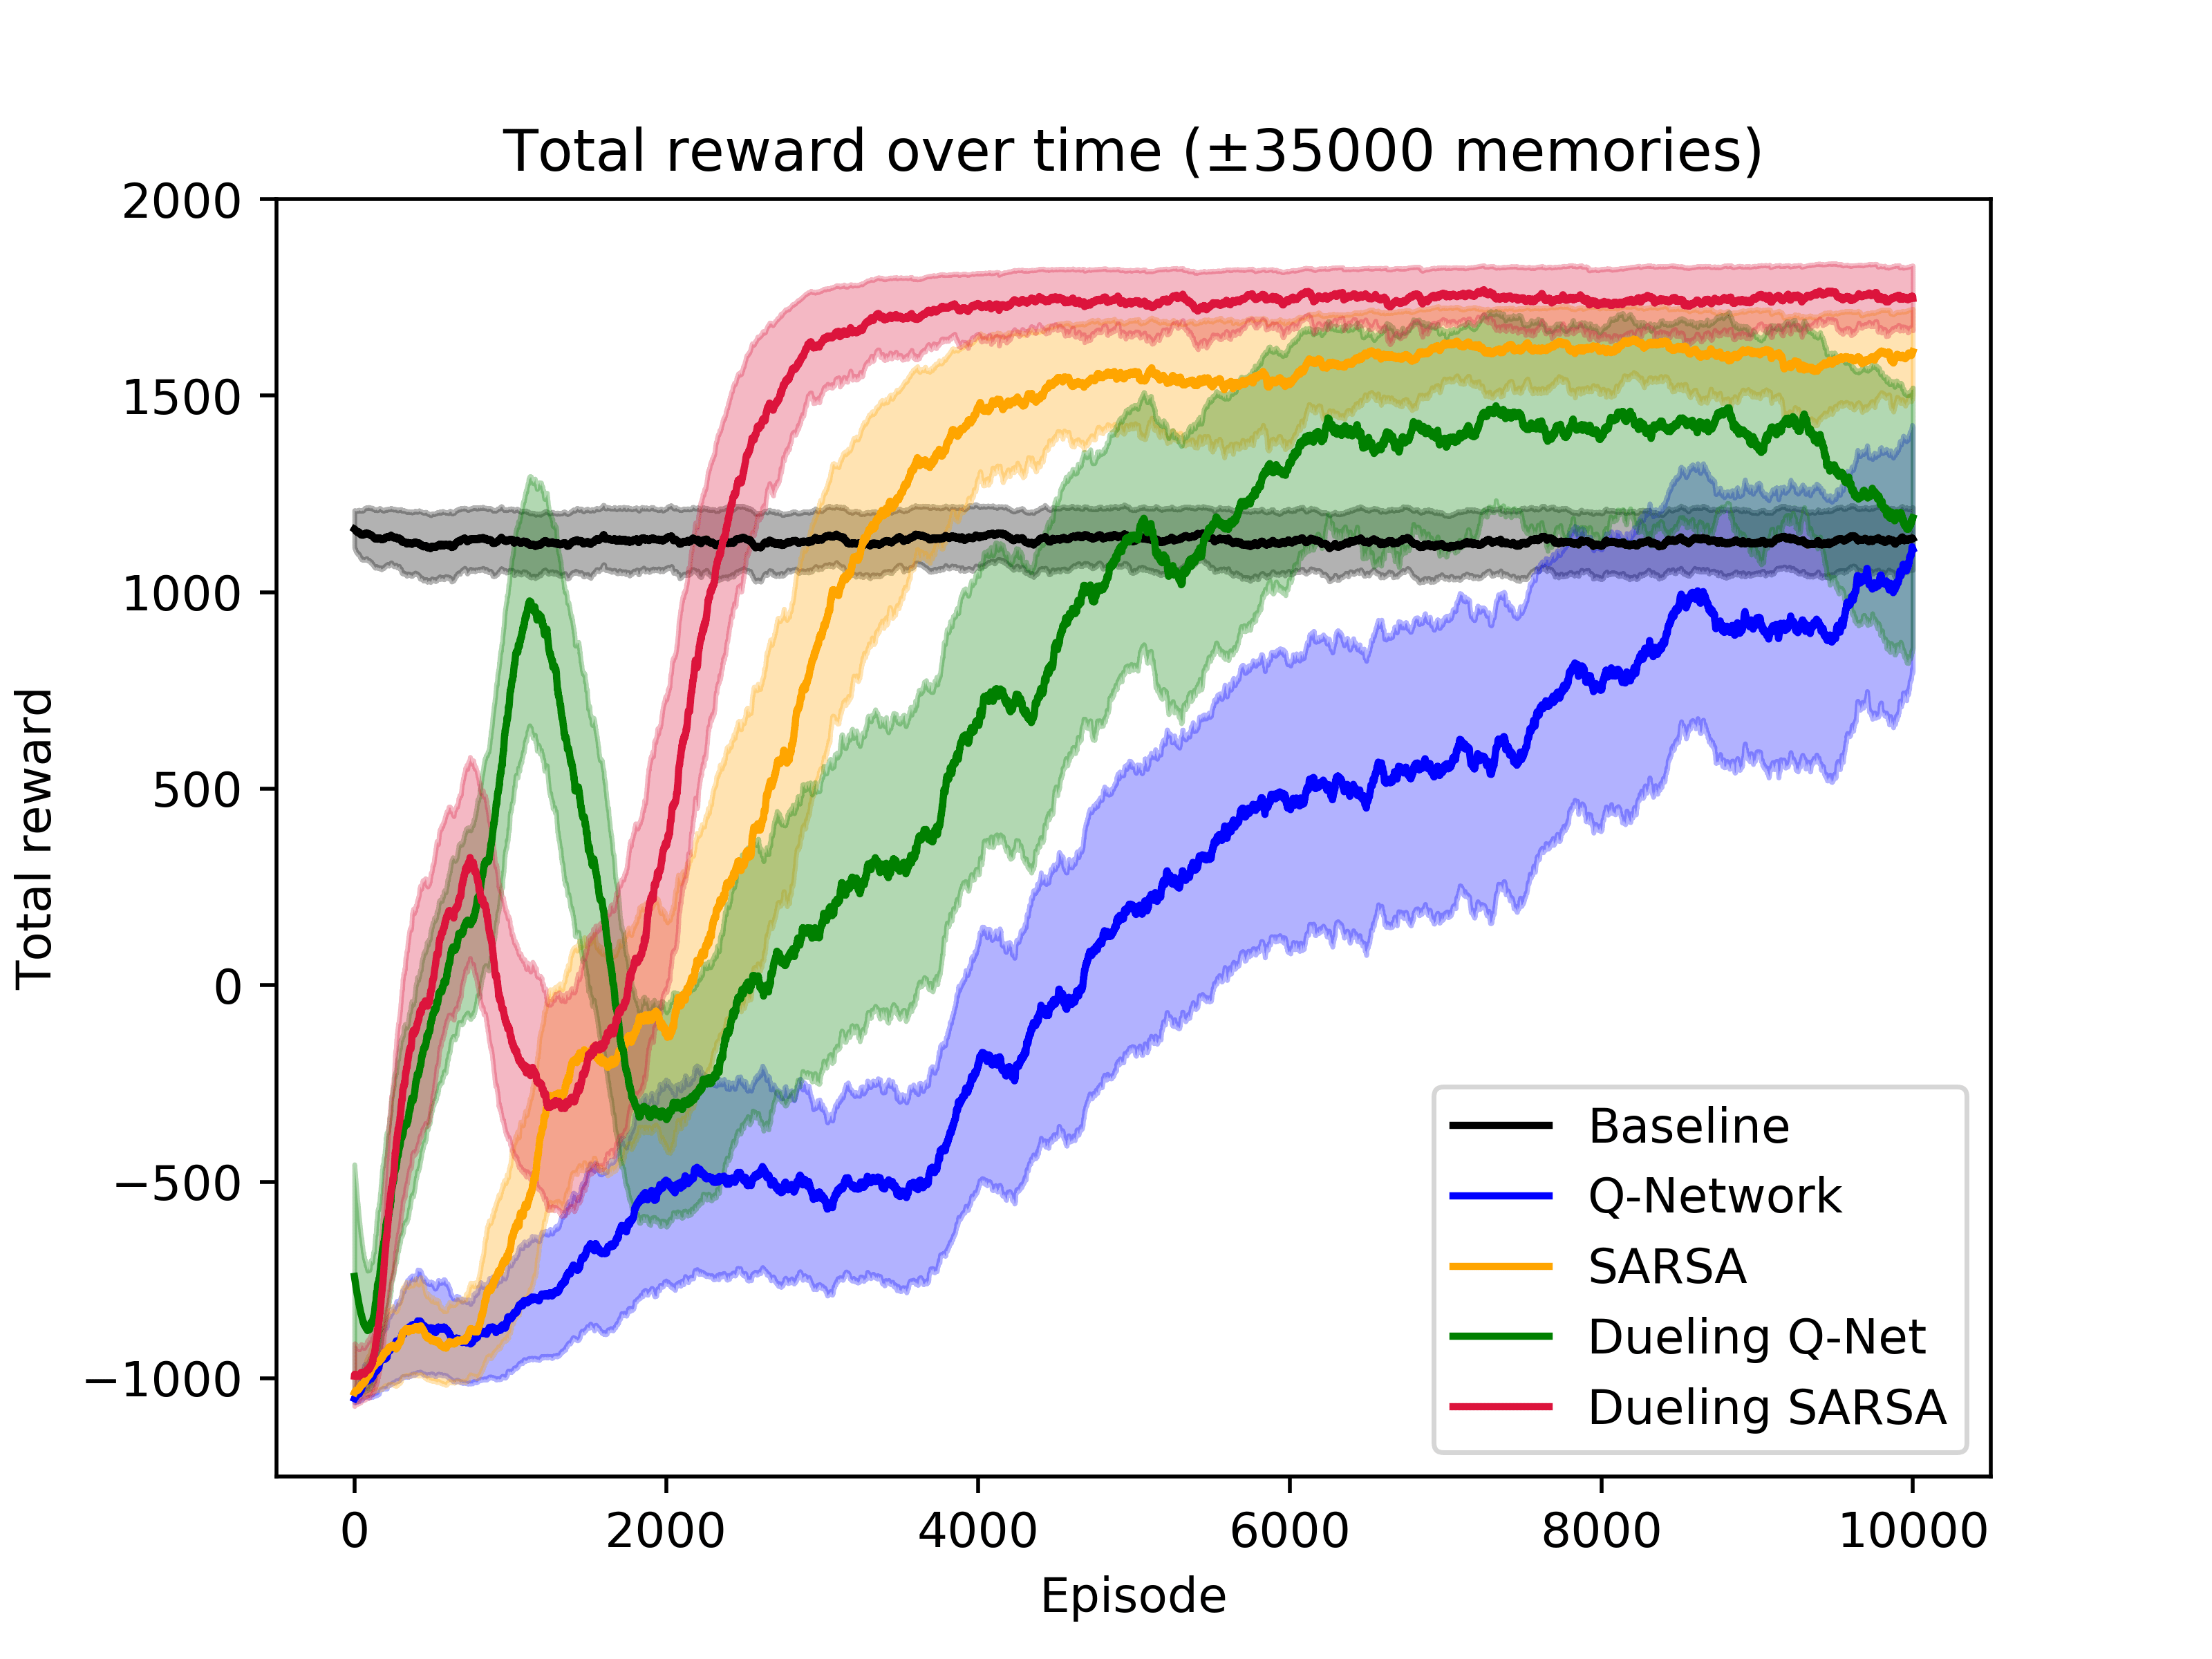
\includegraphics[width=\linewidth]{img/results/10-sized/total_rewards_1000m-min.png}
    \caption{10-by-10 grid given 1000 episodes of demonstation data.}
    \label{fig:10sized-1000mem}
\end{figure}
\hspace{1cm} %Fixes misalignment
\begin{figure}[H]
    \centering
    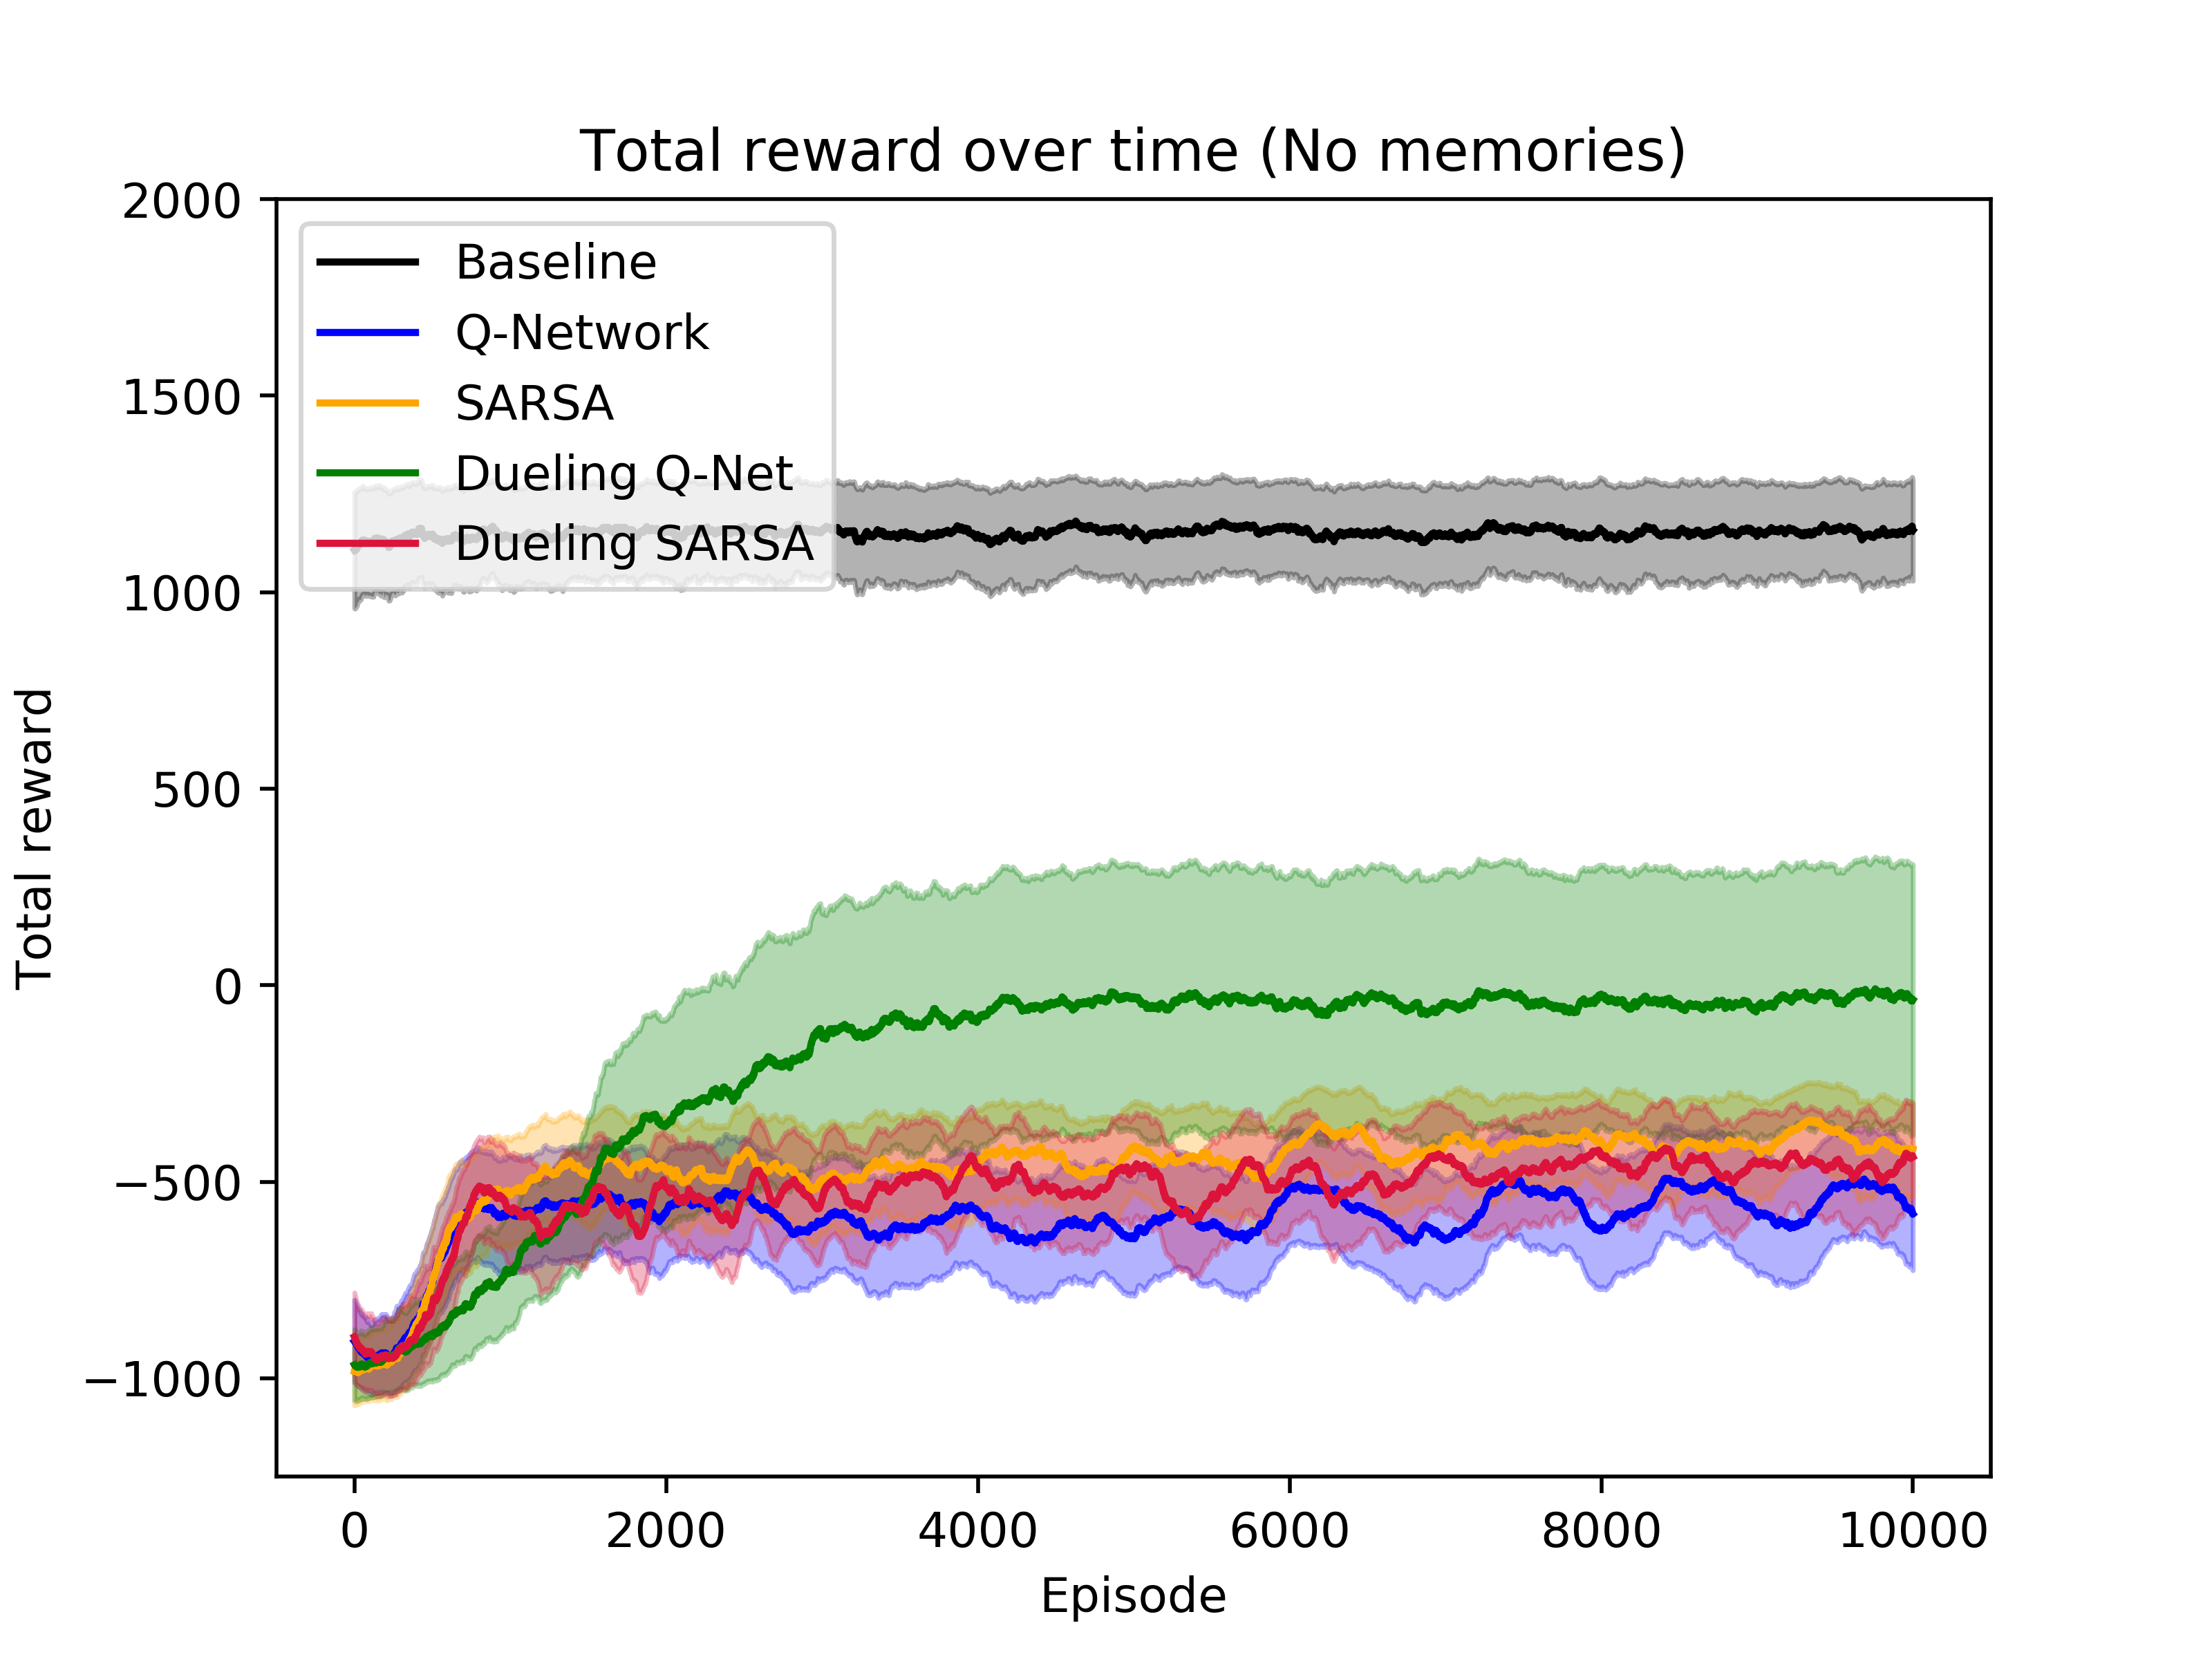
\includegraphics[width=\linewidth]{img/results/14-sized/total_rewards_0m-min.png}
    \caption{14-by-14 grid given no demonstation data.}
    \label{fig:14sized-nomem}
    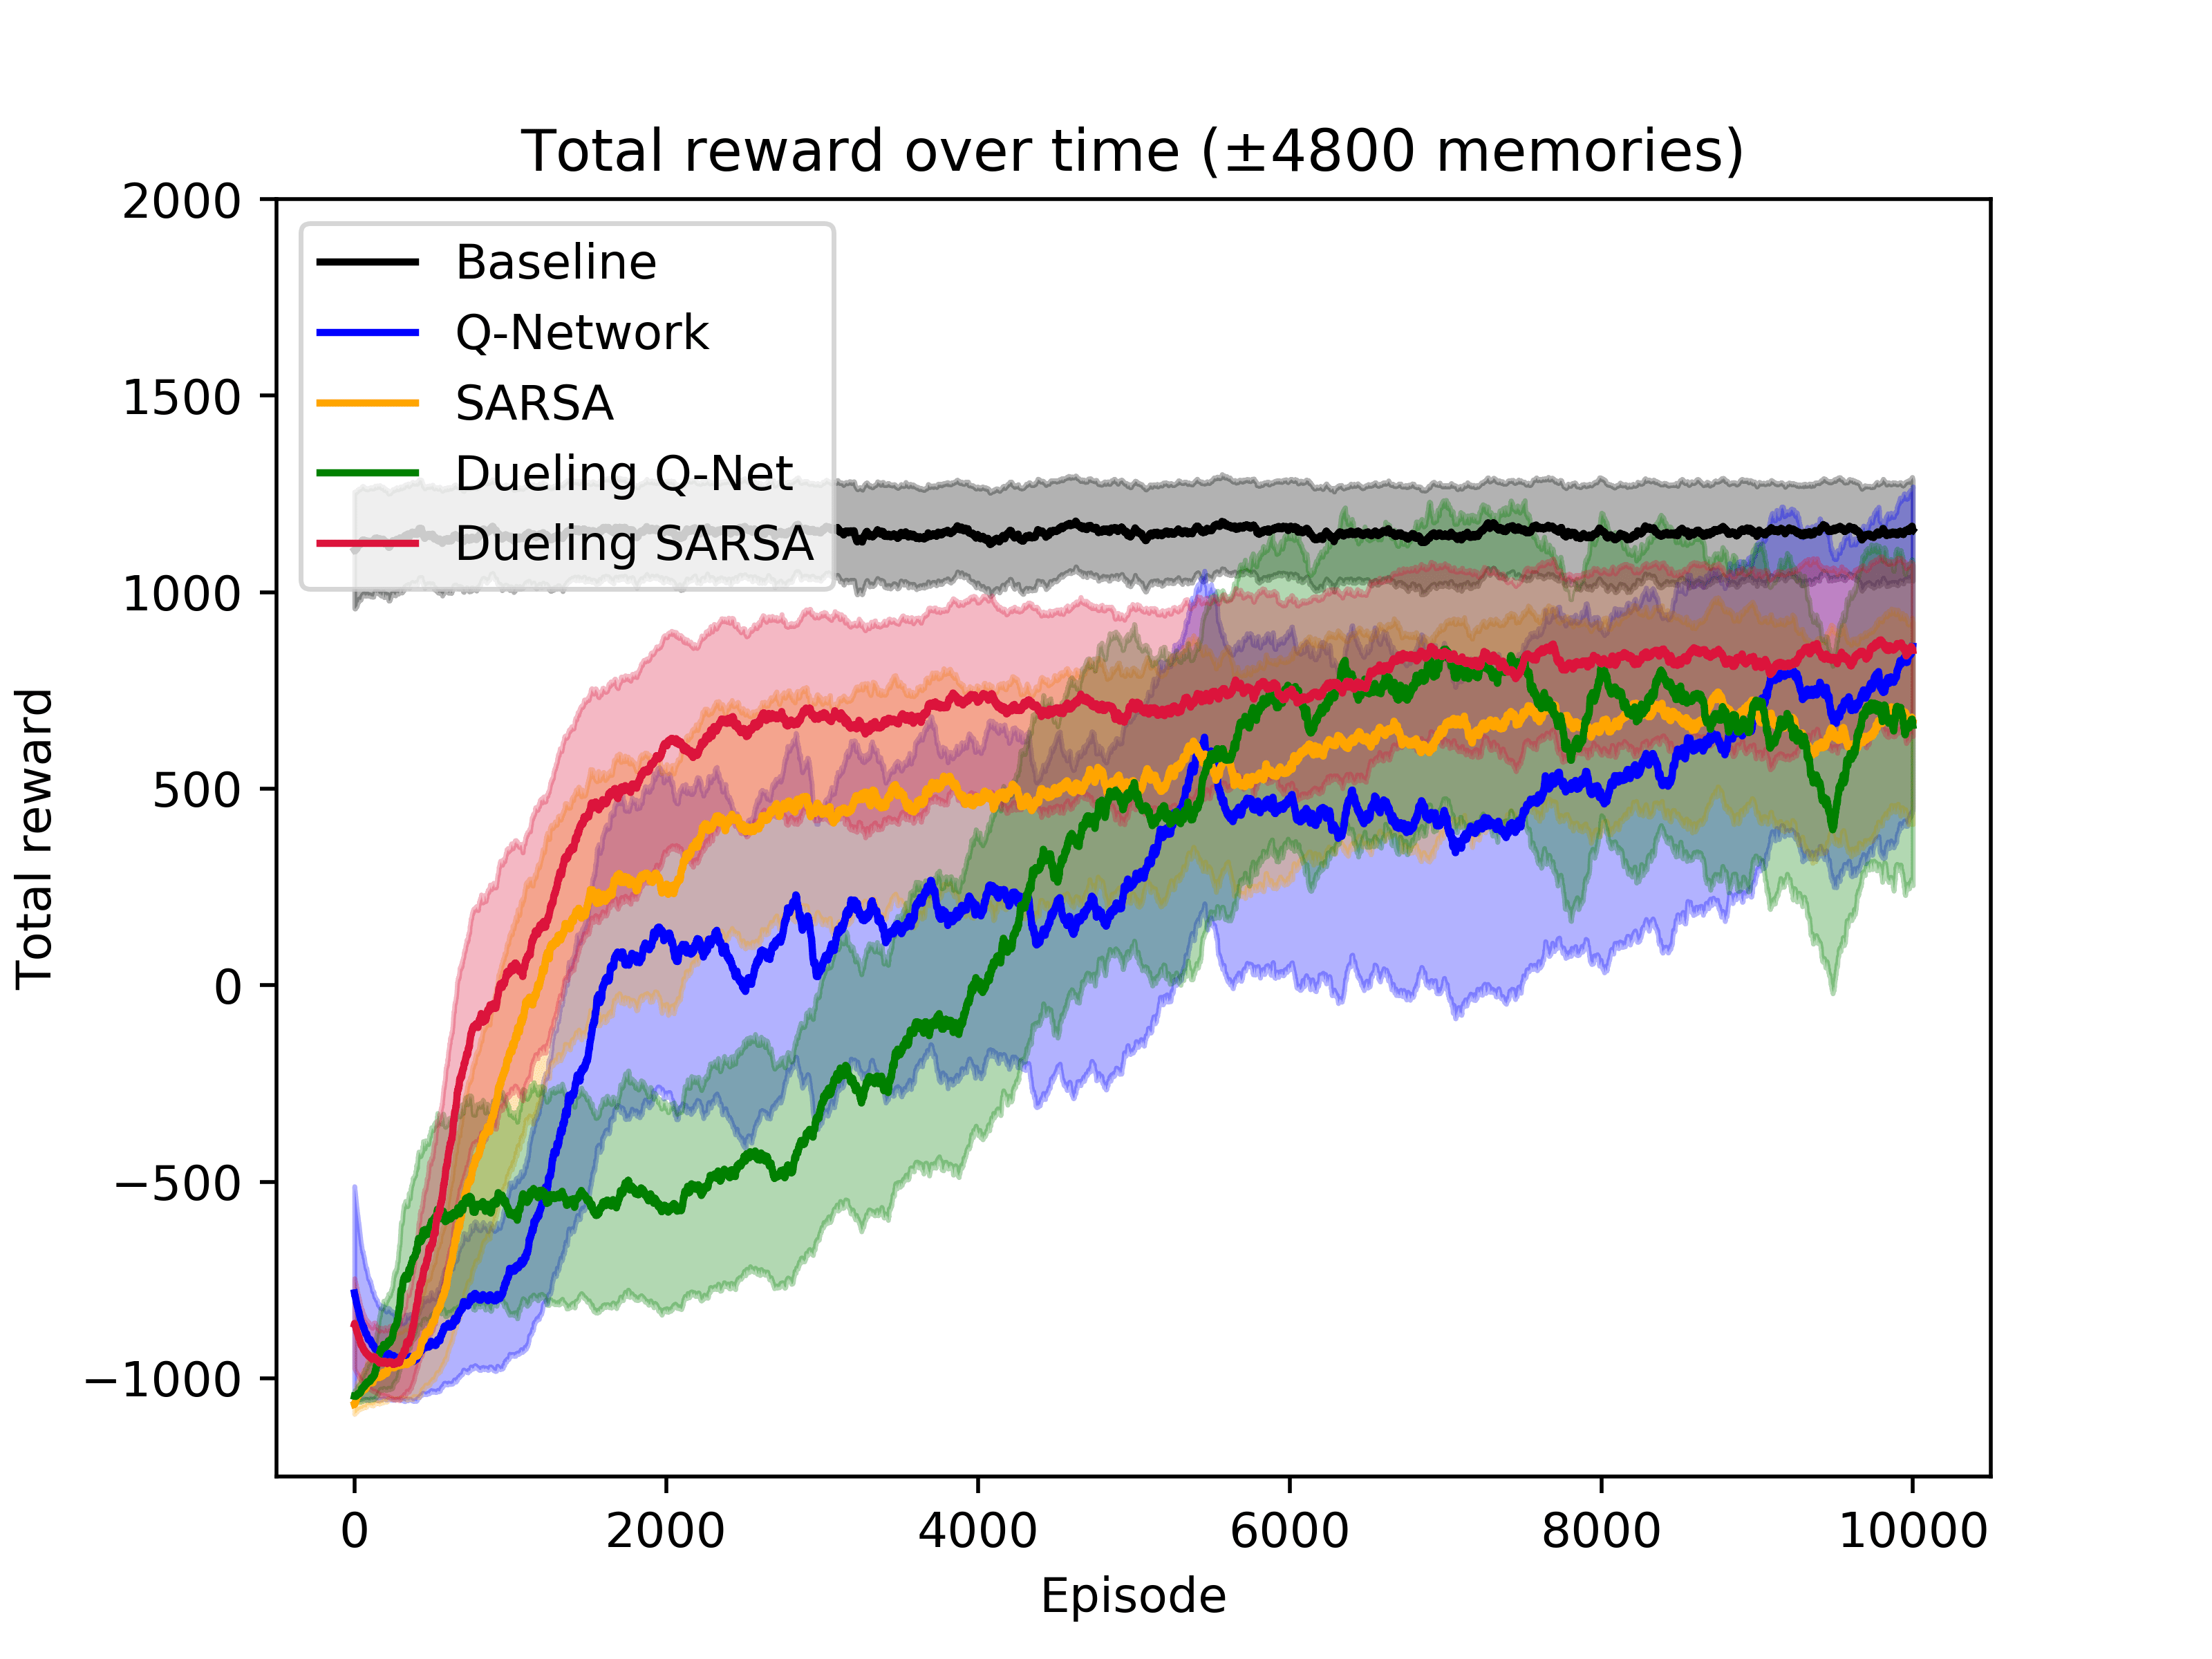
\includegraphics[width=\linewidth]{img/results/14-sized/total_rewards_100m-min.png}
    \caption{14-by-14 grid given 100 episodes of demonstation data.}
    \label{fig:14sized-100mem}
    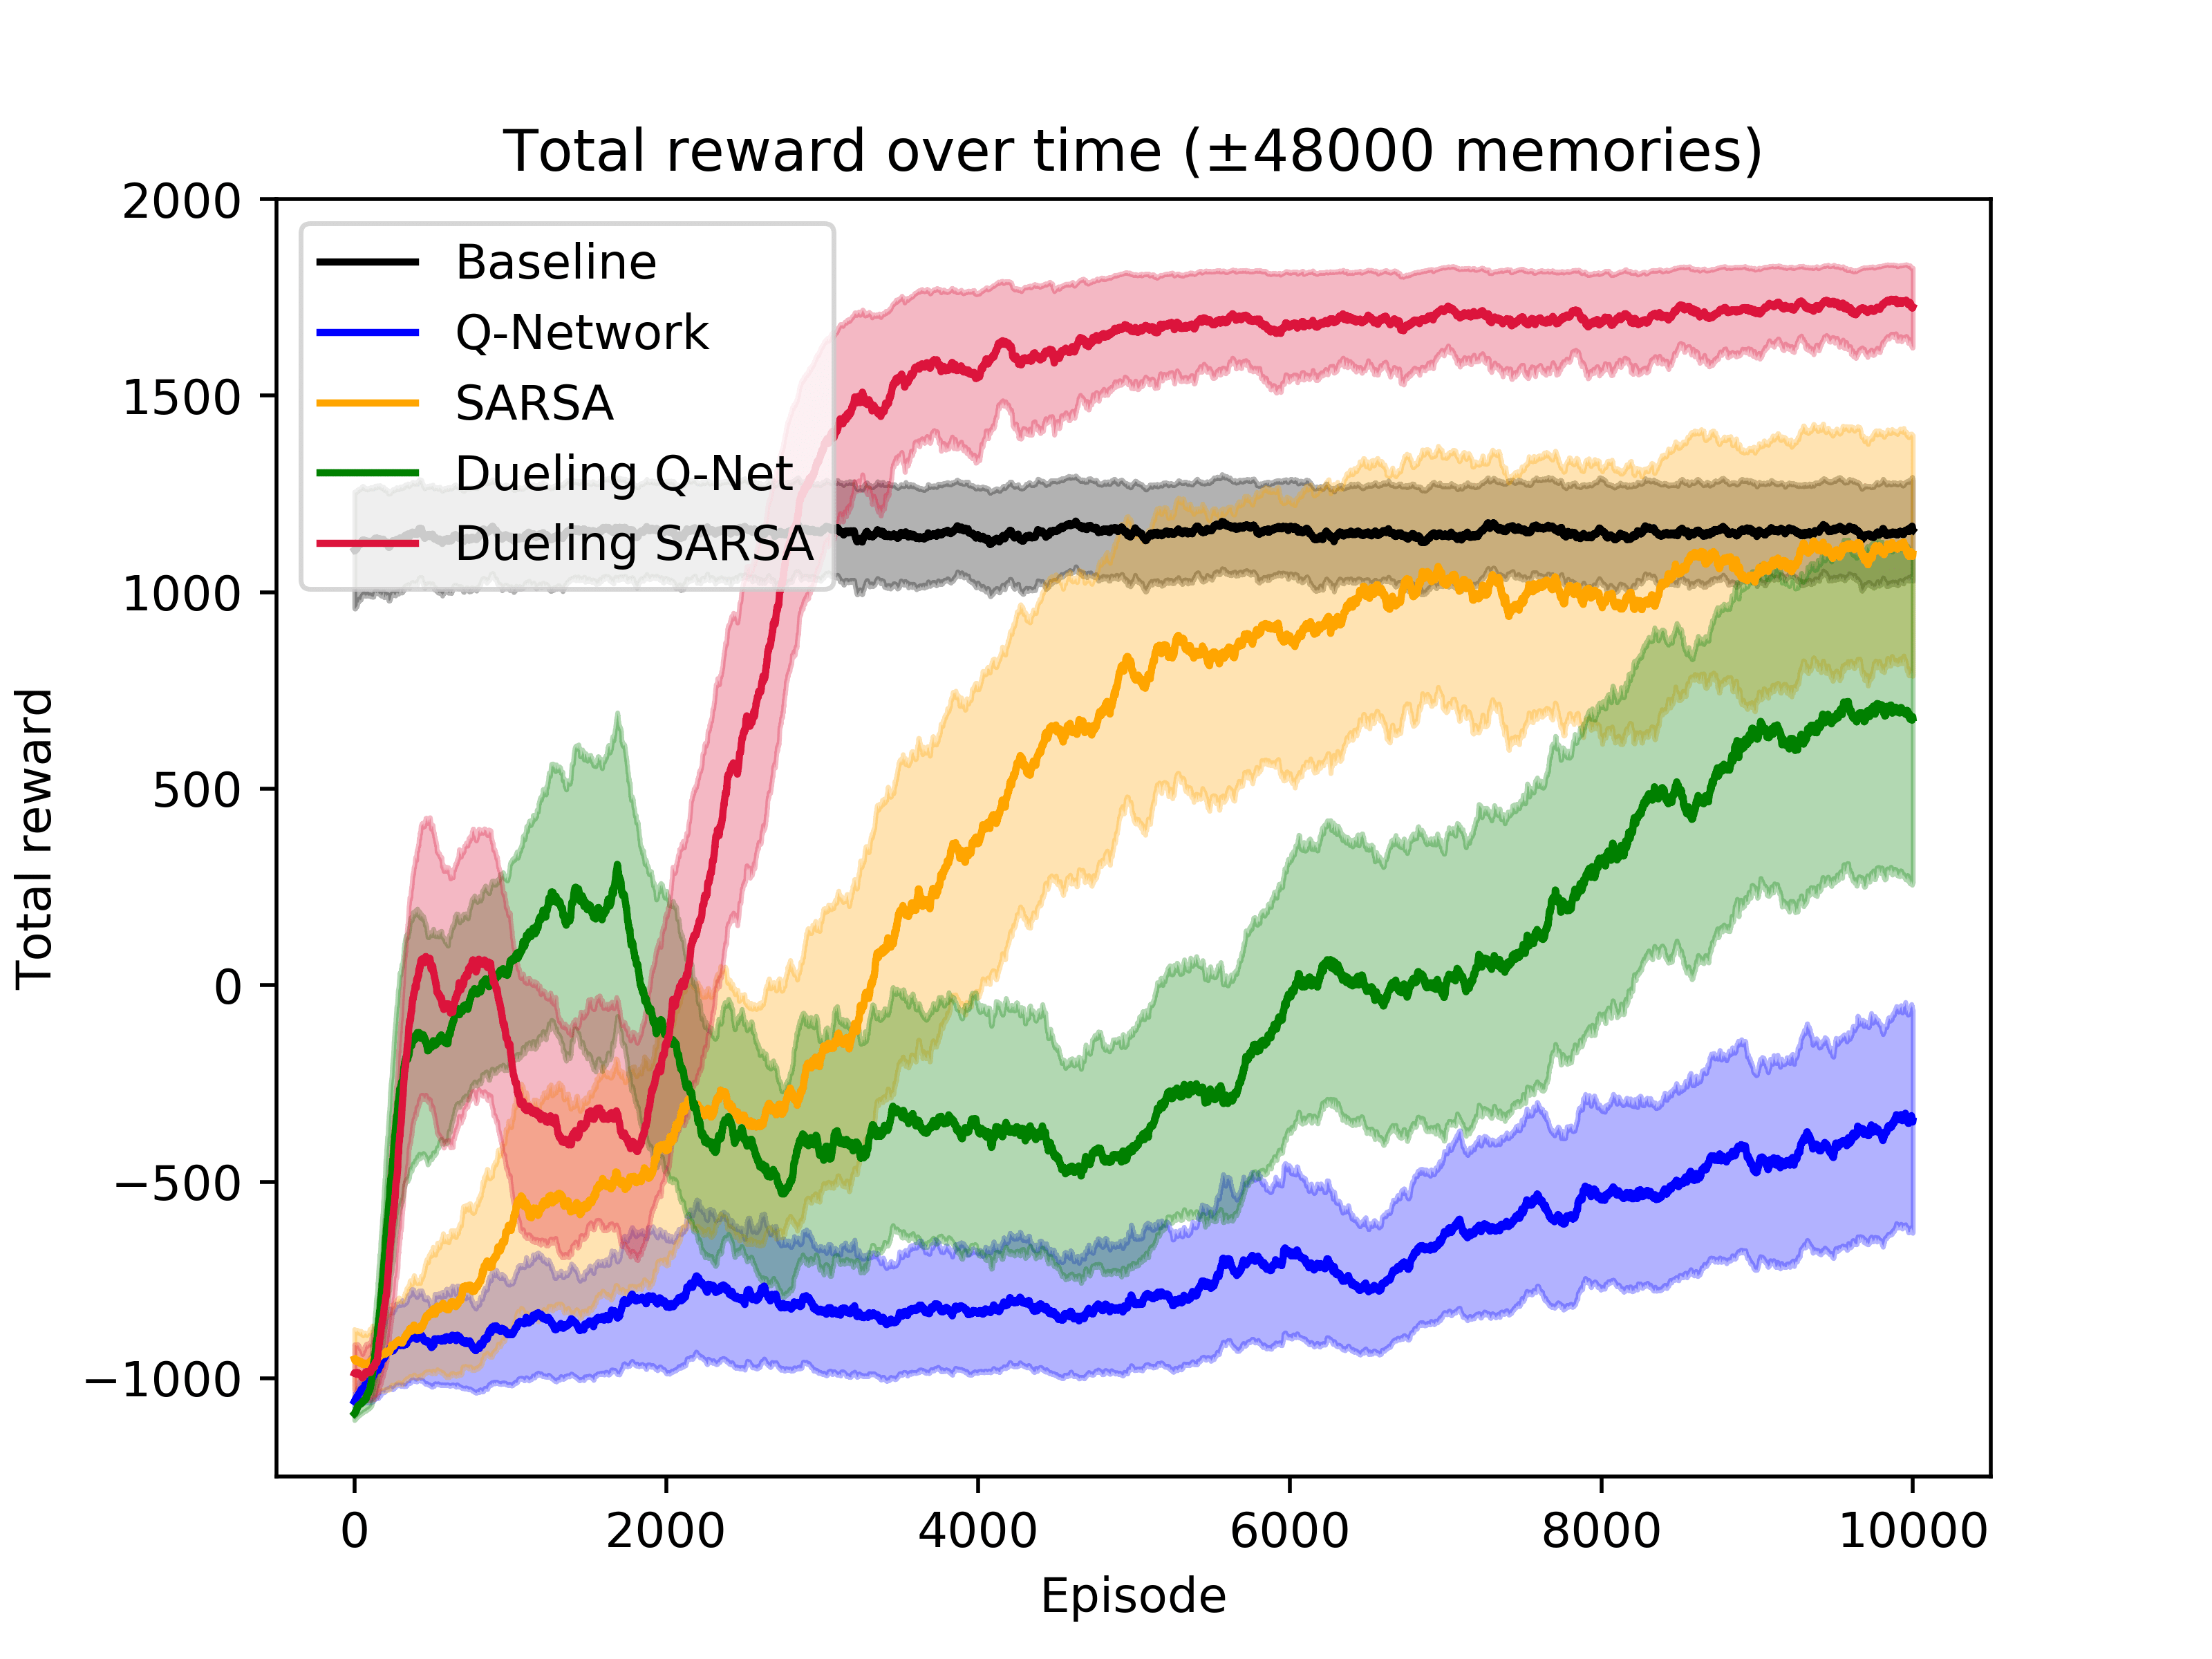
\includegraphics[width=\linewidth]{img/results/14-sized/total_rewards_1000m-min.png}
    \caption{14-by-14 grid given 1000 episodes of demonstation data.}
    \label{fig:14sized-1000mem}
\end{figure}


% SECOND-GEN TABLES
\begin{table}[H]
\begin{tabular}{l|l|l|l|}
\cline{2-4}
\textbf{} & Average Reward & Standard Error & Best Reward \\ \hline
\multicolumn{1}{|l|}{Size 10, no memories} & 1129 & 1.9 & 1387 \\ \hline
\multicolumn{1}{|l|}{Size 10, 100 memories} & 1129 & 1.9 & 1387 \\ \hline
\multicolumn{1}{|l|}{Size 10, 1000 memories} & 1129 & 1.9 & 1387 \\ \hline
\multicolumn{1}{|l|}{Size 14, no memories} & 1152 & 2.8 & 1513 \\ \hline
\multicolumn{1}{|l|}{Size 14, 100 memories} & 1152 & 2.8 & 1513 \\ \hline
\multicolumn{1}{|l|}{Size 14, 1000 memories} & 1152 & 2.8 & 1513 \\ \hline
\end{tabular}
\caption{Baseline rewards of the final 2500 episodes.}
\label{tab:2500base}
\end{table}
\begin{table}[H]
\begin{tabular}{l|l|l|l|}
\cline{2-4}
\textbf{} & Average Reward & Standard Error & Best Reward \\ \hline
\multicolumn{1}{|l|}{Size 10, no memories} & 221 & 4.2 & 715 \\ \hline
\multicolumn{1}{|l|}{Size 10, 100 memories} & 878 & 7.5 & \textbf{1758} \\ \hline
\multicolumn{1}{|l|}{Size 10, 1000 memories} & 907 & 6.7 & \textbf{1696} \\ \hline
\multicolumn{1}{|l|}{Size 14, no memories} & -550 & 2.9 & -139 \\ \hline
\multicolumn{1}{|l|}{Size 14, 100 memories} & 652 & 7.0 & \textbf{1629} \\ \hline
\multicolumn{1}{|l|}{Size 14, 1000 memories} & -459 & 5.0 & 411 \\ \hline
\end{tabular}
\caption{Q-Network rewards of the final 2500 episodes.}
\label{tab:2500qnet}
\end{table}
\begin{table}[H]
\begin{tabular}{l|l|l|l|}
\cline{2-4}
\textbf{} & Average Reward & Standard Error & Best Reward \\ \hline
\multicolumn{1}{|l|}{Size 10, no memories} & 956 & 4.1 & 1335 \\ \hline
\multicolumn{1}{|l|}{Size 10, 100 memories} & 521 & 6.8 & \textbf{1535} \\ \hline
\multicolumn{1}{|l|}{Size 10, 1000 memories} & \textbf{1369} & 5.5 & \textbf{1826} \\ \hline
\multicolumn{1}{|l|}{Size 14, no memories} & -40 & 3.0 & 349 \\ \hline
\multicolumn{1}{|l|}{Size 14, 100 memories} & 667 & 7.8 & \textbf{1748} \\ \hline
\multicolumn{1}{|l|}{Size 14, 1000 memories} & 522 & 7.7 & \textbf{1534} \\ \hline
\end{tabular}
\caption{Dueling Q-Network rewards of the final 2500 episodes.}
\label{tab:2500duel}
\end{table}
\begin{table}[H]
\begin{tabular}{l|l|l|l|}
\cline{2-4}
\textbf{} & Average Reward & Standard Error & Best Reward \\ \hline
\multicolumn{1}{|l|}{Size 10, no memories} & 132 & 3.9 & 563 \\ \hline
\multicolumn{1}{|l|}{Size 10, 100 memories} & 776 & 4.7 & 1292 \\ \hline
\multicolumn{1}{|l|}{Size 10, 1000 memories} & \textbf{1607} & 2.8 & \textbf{1748} \\ \hline
\multicolumn{1}{|l|}{Size 14, no memories} & -398 & 2.4 & -92 \\ \hline
\multicolumn{1}{|l|}{Size 14, 100 memories} & 670 & 5.3 & 1275 \\ \hline
\multicolumn{1}{|l|}{Size 14, 1000 memories} & 1057 & 5.6 & \textbf{1626} \\ \hline
\end{tabular}
\caption{SARSA rewards of the final 2500 episodes.}
\label{tab:2500sarsa}
\end{table}
\clearpage
\begin{table}[H]
\begin{tabular}{l|l|l|l|}
\cline{2-4}
\textbf{} & Average Reward & Standard Error & Best Reward \\ \hline
\multicolumn{1}{|l|}{Size 10, no memories} & 241 & 2.6 & 582 \\ \hline
\multicolumn{1}{|l|}{Size 10, 100 memories} & 1031 & 3.4 & 1312 \\ \hline
\multicolumn{1}{|l|}{Size 10, 1000 memories} & \textbf{1745} & 2.5 & \textbf{1860} \\ \hline
\multicolumn{1}{|l|}{Size 14, no memories} & -455 & 2.6 & -44 \\ \hline
\multicolumn{1}{|l|}{Size 14, 100 memories} & 836 & 4.1 & 1249 \\ \hline
\multicolumn{1}{|l|}{Size 14, 1000 memories} & \textbf{1713} & 3.0 & \textbf{1846} \\ \hline
\end{tabular}
\caption{Dueling SARSA rewards of the final 2500 episodes.}
\label{tab:2500both}
\end{table}


% HYPERPARAMETERS
\begin{table}[H]
\begin{tabular}{|l|l|}
\hline
Memory size & 20000 \\ \hline
Batch size & 32 \\ \hline
Target update (C) & 20 \\ \hline
Gamma (X) & 0.999 \\ \hline
Alpha (X) & 0.005 \\ \hline
Epsilon decay (X) & 0.01 \\ \hline
Epsilon minimum & 1 \\ \hline
Epsilon maximum & 0.005 \\ \hline
\end{tabular}
\caption{All relevant hyper-parameters used in the training process.}
\label{tab:hyperparameters}
\end{table}


\clearpage
\section*{Probably exclude these..}
% FIRST-GEN TABLES
\begin{table}[H]
\begin{tabular}{|l|r|r|r|r|r|}
\hline
\textbf{Experiment Setup} & \multicolumn{1}{l|}{\textbf{Baseline}} & \multicolumn{1}{l|}{\textbf{Q-Network}} & \multicolumn{1}{l|}{\textbf{SARSA}} & \multicolumn{1}{l|}{\textbf{\begin{tabular}[c]{@{}l@{}}Dueling\\ Q-Network\end{tabular}}} & \multicolumn{1}{l|}{\textbf{\begin{tabular}[c]{@{}l@{}}Dueling\\ SARSA\end{tabular}}} \\ \hline
Size 10, no memories & 1130.2 & -81.5 & -149.6 & 692.1 & -9.4 \\ \hline
Size 10, 100 memories & 1130.2 & 869.0 & 642.5 & 470.7 & 845.4 \\ \hline
Size 10, 1000 memories & 1130.2 & 98.9 & 1017.5 & 825.6 & \textbf{1333.9} \\ \hline
Size 14, no memories & 1151.4 & -590.5 & -460.9 & -188.8 & -523.2 \\ \hline
Size 14, 100 memories & 1151.4 & -220.5 & 412.6 & 197.4 & 604.5 \\ \hline
Size 14, 1000 memories & 1151.4 & -708.8 & 421.8 & -11.8 & \textbf{1194.0} \\ \hline
\end{tabular}
\caption{Averaged rewards from all training episodes.}
\label{tab:averages}
\end{table}
\begin{table}[H]
\begin{tabular}{|l|r|r|r|r|r|}
\hline
\textbf{Experiment Setup} & \multicolumn{1}{l|}{\textbf{Baseline}} & \multicolumn{1}{l|}{\textbf{Q-Network}} & \multicolumn{1}{l|}{\textbf{SARSA}} & \multicolumn{1}{l|}{\textbf{\begin{tabular}[c]{@{}l@{}}Dueling\\ Q-Network\end{tabular}}} & \multicolumn{1}{l|}{\textbf{\begin{tabular}[c]{@{}l@{}}Dueling\\ SARSA\end{tabular}}} \\ \hline
Size 10, no memories & 1265.8 & 435.7 & 327.0 & 1187.8 & 382.0 \\ \hline
Size 10, 100 memories & 1265.8 & \textbf{1608.8} & 1159.1 & \textbf{1272.0} & 1255.1 \\ \hline
Size 10, 1000 memories & 1265.8 & 1243.7 & \textbf{1726.6} & \textbf{1730.8} & \textbf{1832.6} \\ \hline
Size 14, no memories & 1363.4 & -326.3 & -226.2 & 177.5 & -262.7 \\ \hline
Size 14, 100 memories & 1363.4 & 1049.0 & 1028.0 & 1225.5 & 1112.0 \\ \hline
Size 14, 1000 memories & 1363.4 & -181.3 & \textbf{1393.9} & 912.5 & \textbf{1830.2} \\ \hline
\end{tabular}
\caption{Averaged rewards from the best 1000 training episodes.}
\label{tab:best10averages}
\end{table}
\begin{table}[H]
\begin{tabular}{|l|r|r|r|r|r|}
\hline
\textbf{Experiment Setup} & \multicolumn{1}{l|}{\textbf{Baseline}} & \multicolumn{1}{l|}{\textbf{Q-Network}} & \multicolumn{1}{l|}{\textbf{SARSA}} & \multicolumn{1}{l|}{\textbf{\begin{tabular}[c]{@{}l@{}}Dueling\\ Q-Network\end{tabular}}} & \multicolumn{1}{l|}{\textbf{\begin{tabular}[c]{@{}l@{}}Dueling\\ SARSA\end{tabular}}} \\ \hline
Size 10, no memories & 1132.3 & 253.6 & 180.5 & 973.4 & 255.0 \\ \hline
Size 10, 100 memories & 1132.3 & 692.5 & 791.5 & 548.3 & 1040.7 \\ \hline
Size 10, 1000 memories & 1132.3 & 977.2 & \textbf{1591.9} & \textbf{1297.5} & \textbf{1751.3} \\ \hline
Size 14, no memories & 1155.4 & -551.0 & -391.5 & -28.1 & -457.0 \\ \hline
Size 14, 100 memories & 1155.4 & 772.7 & 647.1 & 614.0 & 841.6 \\ \hline
Size 14, 1000 memories & 1155.4 & -387.3 & 1102.7 & 674.4 & \textbf{1729.1} \\ \hline
\end{tabular}
\caption{Averaged rewards from the final 1000 training episodes.}
\label{tab:last10averages}
\end{table}
    \newpage
\end{appendices}

\end{document}
